%!TEX root = ../thesis.tex
%*******************************************************************************
%*********************************** First Chapter *****************************
%*******************************************************************************

\chapter{Variant discovery in genome graphs}
\label{chap:denovo}
\ifpdf
    \graphicspath{{Chapter1/Figs/Raster/}{Chapter1/Figs/PDF/}{Chapter1/Figs/}}
\else
    \graphicspath{{Chapter1/Figs/Vector/}{Chapter1/Figs/}}
\fi
% ==================================================================
\setcounter{section}{-1}
\section{Publication and collaboration acknowledgements}
\label{sec:denovo-acknowledge}

% ==================================================================
\section{Introduction}

% ==================================================================
\section{Methods}
\label{sec:denovo-method}

We define a method that extends \pandora{}, with a subcommand \vrb{discover}, to allow for the \denovo{} discovery of variants not present a \prg{}. It is implemented within the \pandora{} code base, in the C++ programming language. 

The first step of \denovo{} variant discovery in genome graphs is finding the candidate regions of the graph that show evidence of dissimilarity from the sample's reads.

\subsection{Finding candidate regions}

The input required for finding candidate regions are a local \prg{} (node), $n$, within the \pandora{} \panrg{}; the maximum likelihood path of both sequence and \kmer{}s in $n$, $lmp_n$ and $kmp_n$ respectively; and a padding size, $w$, for the number of positions surrounding the candidate region to retrieve.

We define a candidate region, $r$, as an interval within $n$ where read depth (coverage) on $lmp_n$ is less than a given threshold, $c$, for more than $l$ and less than $m$ consecutive positions. We note that coverage is actually stored on $kmp_n$, but is stored for the whole \kmer{}. We convert the coverage on $kmp_n$ into per-position coverage on $lmp_n$ and use that for identifying low-coverage segments as just described. $m$ acts to restrict the size of variants we are able to detect. If set too large, the following steps become much slower due to the combinatorial expansion of possible paths. 

For a given read, $s$, that has a mapping to $r$, we define $s_r$ to be the subsequence of $s$ that maps to $r$, including an extra $w$ positions either side of the mapping. We define the pileup $P_r$ as the set of all $s_r \in r$.

\subsection{Enumerating paths through candidate regions}
\label{sec:path-enum}

For $r \in R$, where $R$ is the set of all candidate regions, we construct a de Bruijn graph $G_r$ from $P_r$ using the GATB library \cite{gatb2014}. 

$A_L$ and $A_R$ are defined as sets of \kmer{}s to the left and right of $r$ in the maximum likelihood path $lmp_n$. They are anchors to allow insertion of new sequences found by \denovo{} discovery into the local \prg{}. Each set has a maximum size of $k$.

We abandon \denovo{} discovery if $A_L \cap G_r = \emptyset \lor A_R \cap G_r = \emptyset$. That is, if no pairwise combination of left and right anchor \kmer{}s exists in the de Bruijn graph $G_r$.

We use sets of \kmer{}s for $A_L$ and $A_R$, rather than a single anchor \kmer{}, to provide redundancy in the case where sequencing errors cause some anchors to not be in $G_r$. We define the start anchor \kmer{}, $a_L$, as the first (left-most) $a_L \in A_L \land a_L \in G_r$. Likewise, we define the end anchor \kmer{}, $a_R$, as the left-most $a_R \in A_R \land a_R \in G_r$.

Now that we have two anchor \kmer{}s, $a_L$ and $a_R$, our goal is to find all (valid) paths between these anchors in the de Bruijn graph ($G_r$).

$T_r$ is the spanning tree obtained by performing depth-first search (DFS) on $G_r$, beginning from $a_L$. $p_r$ is defined as a path, from the root node $a_L$ of $T_r$ and ending at node $a_R$, which fulfils the following two conditions:

\begin{enumerate}
  \item $p_r$ is shorter than the maximum allowed path length.
  \item No more than $k$ nodes along $p_r$ have coverage $< (0.1 n_r e_r)$, where $e_r$ is the expected \kmer{} coverage for $r$ and $n_r$ is the number of iterations of path enumeration for $r$.
\end{enumerate}

$V_r$ is the set of all $p_r$. If $|V_r|$ is greater than a predefined threshold, $n_r$ is incremented by 1 and $V_r$ is repopulated. If $0.1n_r = 1.0$ then \denovo{} discovery is abandoned for $r$.

The second condition listed above, which relies on $n_r$ and $e_r$ has the effect of progressively increasing the amount of coverage we demand on a candidate path ($p_r$). In the first iteration, $n_r=1$, therefore we require the path has 10\% of the expected read depth (coverage). If this yields too many paths (condition 1), we restart and require all paths to have 20\% of the expected coverage. If we reach a stage where we require 100\% of the expected coverage, but still have too many paths, we quit \denovo{} discovery for the candidate region.

\subsubsection{Pruning the path-space in a candidate region}

As \pandora{} operates on both accurate and error-prone sequencing reads, the number of valid paths in $G_r$ can be very large. In testing, we found the path enumeration process can result in runtimes beyond seven days in some scenarios. The increased runtime is due to cycles that can occur in $G_r$ and exploring paths that will never reach our required end anchor ($a_R$). 

In order to reduce the path-space within $G_r$, we prune paths based on multiple criteria. Critically, this pruning happens at each step of the graph walk (path-building; \autoref{sec:path-enum}).

In addition to $T_r$, obtained by performing DFS on $G_r$, we produce a distance map $D_r$ that results from running reversed breadth-first search (BFS) on $G_r$, beginning from \emph{the end anchor} ($a_R$). We say reversed BFS as we explore the \emph{predecessors} of each node, rather than the successors. $D_r$ is implemented as a binary search tree where each node in the tree represents a \kmer{} in $G_r$ that is reachable from $a_R$ via reversed BFS. Each node additionally has an integer attached to it that describes the shortest path from that node to $a_R$.

We can use $D_r$ to prune the path-space as follows. As we walk (enumerate) the candidate path ($p_r$) in \autoref{sec:path-enum}, for each node (\kmer{}; $v$) in $G_r$, starting at $a_L$, we check if $a_R$ be reached from $v$ in a minimum of $i$ nodes, where $i$ is defined as the maximum allowed path length minus the number of nodes walked to reach $v$. If one of these conditions is not met, we abandon $p_r$. 

The advantage of this pruning process is that we never explore paths that will not reach our required end point. Additionally, we will discard any path once we have made too many loops around a graph cycle.

\noindent
In the end, for each candidate region ($r$), we are left with a collection of paths ($V_r$) between two \kmer{}s ($a_L$ and $a_R$). We create the final candidate paths by replacing the sequence between $a_L$ and $a_R$ in the maximum likelihood path ($lmp_n$) with each path ($p_r$) in $V_r$. These are written to file - with one file per candidate region. Padding the candidate paths in this way ensures they are inserted into the \prg{} in the correct location (see \autoref{sec:denovo-insert}). 

\subsection{Updating a \panrg{} with candidate paths}
\label{sec:denovo-insert}

As new paths alter the structure of a \prg{}, we cannot insert them directly, and must rebuild each \prg{} for which a candidate path is discovered.

The first step of rebuilding each local \prg{} is to add the new candidate paths to the original multiple sequence alignment (MSA). Because we padded each path with the maximum likelihood path, this ensures the novel path aligns with the correct section of the locus. We combine all candidate paths for a locus into a single, unaligned FASTA file and add them to the existing locus MSA with the \vrb{--add} routine in MAFFT \cite{katoh2012}. 

Next, \makeprg{} is run on the subsequent alignments, and the resulting updated local \prg{}s are combined into a single \panrg{} and indexed with \pandora{}. 

This updated \panrg{} can then be used as input to \pandora{} and subsequent genotyping will include the novel variants.

% ==================================================================
\section{Simulation data}
\label{sec:denovo-sims}
Having described an extension of the \pandora{} program that allows for \denovo{} variant discovery, we now turn our attention to its evaluation.

\subsection{Methods}
\label{sec:denovo-sims-methods}

The first step in evaluating the effect of adding \denovo{} variant calling to \pandora{} is with a simulated dataset. We aim to show that the addition of \denovo{} discovery allows \pandora{} to improve its probability of variant detection (recall) with minimal impact on the quality of the calls (precision). 

To construct our simulated dataset, we randomly select 100 gene MSAs from a pool of 29,702 obtained for \ecoli{} from the panX database \cite{panx}. Next, a local \prg{} is constructed for each MSA with \makeprg{}. We used a range of maximum nesting levels (\todo[inline]{link to intro section on make prg}) - 1, 3, 5, and 10 - in order to investigate whether \prg{} nesting has an impact on our ability to discover novel variants. The local \prg{}s are combined into a single \panrg{} for each nesting level. A random path through each \prg{} is selected using \pandora{} and concatenated together to form a single "genome" sequence. 

We subsequently add SNPs to the simulated genome at different rates of SNPs per-gene using \vrb{snp-mutator} \cite{snpmutator}. For this work, we introduce 100, 400, and 1,000 SNPs to the simulated genome, which equate to approximately 1, 4, and 10 SNPs per gene, respectively. \vrb{snp-mutator} produces a VCF of the SNPs that were introduced, along with the mutated genome sequence.

Next, we simulated 30,000 \ont{} reads from the mutated genomes using \vrb{nanosim-h} \cite{yang2017,brinda2018}. As the most recent model offered by \vrb{nanosim-h} was from the old R9 \ont{} flow cell, we trained and used a model from a freely-available \ecoli{} R9.4 dataset (\url{http://lab.loman.net/2017/03/09/ultrareads-for-nanopore/}). Each read set was randomly subsampled to a read depth (coverage) of 15, 30, 60, and 100 with \vrb{rasusa} \cite{rasusa2019} so we can investigate the impact of coverage on our ability to discover novel variants.

\pandora{}'s \vrb{discover} routine is then run, using the original panX-derived \panrg{} and the reads simulated from the mutated genome. With this approach, we know that the reads originate from a sequence in our \panrg{}, but with some SNP differences and \ont{} errors. It is possible that some of the random SNPs introduced by \vrb{snp-mutator} already exist in the \panrg{}, but this is likely to be a very small number. We use three different \kmer{} sizes for the \denovo{} discovery: 11, 13, and 15. 

After running the \vrb{discover} routine, we are left with a collection of candidate paths produced by the \denovo{} component. We then add these candidate paths back into the \panrg{} as per \autoref{sec:denovo-insert}. The updated \panrg{} is then used as input - along with the simulated reads - to \pandora{} \vrb{map} to produce a genotyped VCF that hopefully contains all of the simulated SNPs.

In parallel to this, we also run \pandora{} \vrb{map} on the original \panrg{} and simulated reads - i.e., without variant discovery. The genotyped VCF produced by this run shows how \pandora{} performed prior to the addition of \denovo{} variant discovery in this chapter. Theoretically, we only expect this VCF to contain simulated SNPs that were already in the \panrg{}.

At the end of this workflow, we have a genotyped VCF with and without \denovo{} variant discovery for each combination of maximum nesting, \denovo{} \kmer{} size, SNP rate, and read depth (coverage).

\subsection{Evaluation}
\label{sec:denovo-sims-eval}

Comparing the truth VCF to the one produced by \pandora{} requires care. The variants in the truth VCF are with respect to a linear reference genome; as we only simulated SNPs, these are single positions records. However, the \pandora{} variants are with respect to a graph, and depending on the density of variation in the graph, may not appear as single position records (see \autoref{fig:min-match-len-example} for an illustration of this). 

We avoid the error-prone conversion of linear coordinates into graph coordinates, or vice versa, by using a coordinate-free evaluation. This approach maps variant \emph{probes} to each other and compares the probe sequences.  

We define a probe-set $P$ as a collection of probes, $p$, where $p$ represents an entry, $e$, in a VCF file, $V$. For each $e \in V$, $p$ is constructed by the concatenation of $l_w$, $e_c$, and $r_w$ (in that order), where $e_c$ is the called variant of $e$ (alternate allele), and $l_w$ and $r_w$ are the sequences, of maximum length $w$, in the VCF reference to the left and right, respectively, of $e_c$. For \pandora{}, the VCF reference is the maximum likelihood sequence, and for the truth VCF it is the simulated genome (without the simulated SNPs).

A truth probe-set, $P_t$, was constructed from the VCF of variants added to the simulated genome and a query probe-set, $P_q$, from the variants called by \pandora{}. We then mapped all probes from $P_t$ to $P_q$ using \texttt{bwa mem} \cite{li2013}. We classify each probe in $P_t$ as a true positive (TP) if the $e_c$ part of the probe exactly matches the sequence it aligns to in $P_q$, or a false negative (FN) otherwise. Any probe in $P_q$ that does not have a TP truth probe mapped to it is classified as a false positive (FP). We perform this assessment for the pre-\denovo{} (\vrb{no\_denovo}) and post-\denovo{} (\vrb{with\_denovo}) VCF files from \pandora{}. 

Precision is defined as the number of TPs divided by the number of TPs and FPs $precision=\frac{TP}{TP+FP}$; it represents the fraction of variant calls made that are correct. Likewise, recall is calculated as $recall=\frac{TP}{TP+FN}$ and describes the proportion of expected variants correctly discovered.

\subsection{Results}

We first look at \autoref{fig:denovo-sims}, which shows how precision and recall of the \pandora{} \denovo{} variants changes depending on the combination of parameters chosen. Those parameters were the read depth (coverage) of the simulated reads (\autoref{fig:denovo-sims-covg}), the number of SNPs introduced into the simulated genome (\autoref{fig:denovo-sims-num-snps}), the \kmer{} size used for variant discovery (\autoref{fig:denovo-sims-kmer-size}), and the maximum nesting level allowed in the \prg{}s (\autoref{fig:denovo-sims-nesting}). In total, there are 144 different combinations of parameters, and thus data points.

Perhaps the parameter that has the most obvious impact on the precision and recall is the coverage (\autoref{fig:denovo-sims-covg}). It is somewhat unsurprising that as coverage increase, so do both precision and recall. However, there does not seem to be any noticeable difference for coverage $\ge 60$.

In the best case, the highest recall and precision values are 0.91 and 1.0, respectively. In both instances, the data point is the same, with a coverage of 60, \kmer{} size of 13, number of SNPs 100, and a maximum nesting level of 10. Upon further investigation of the 9 missed variants (FNs) for this data point, six were within $2k-1$ positions of the start or end of the locus, one was a null call where the correct variant actually had the highest coverage, one was falsely called as a homopolymer deletion, and the remaining missed call never had \denovo{} discovery triggered for that region of the locus. Therefore, only 3/9 FNs for this example (the last two) were discoverable with our \denovo{} method.

The last point requires some elaboration, as it may not be clear why only three FNs in the best-performing data point were expected to be detected by \denovo{}. In the case of the null genotype call, the correct variant was discovered, and it had higher coverage than the reference allele (26 vs 11), therefore it is a failure of the genotyping. The homopolymer deletion is actually both a failure of \denovo{} and the genotyping; \denovo{} (incorrectly) discovered the candidate indel, but the genotyping confirmed it. And the variant that \denovo{} never triggered \denovo{} discovery most likely has enough coverage on the reference allele that a candidate region was not detected - by default we only flag a candidate region is coverage drops below 3.

In the case of the six missed calls near the ends of loci, these are not detectable by our current \denovo{} method as they occur within $2k-1$ positions of the boundary of a locus. The reason this makes them undetectable is related to our need for start and end anchor \kmer{}s in order to find candidate paths (\autoref{sec:path-enum}). The start and end \kmer{}s are a collection of $k$ \kmer{}s, meaning $2k-1$ positions are required surrounding a candidate region in order to be able to initiate \denovo{} discovery.

\begin{figure}
     \centering
     \begin{subfigure}[b]{0.475\textwidth}
        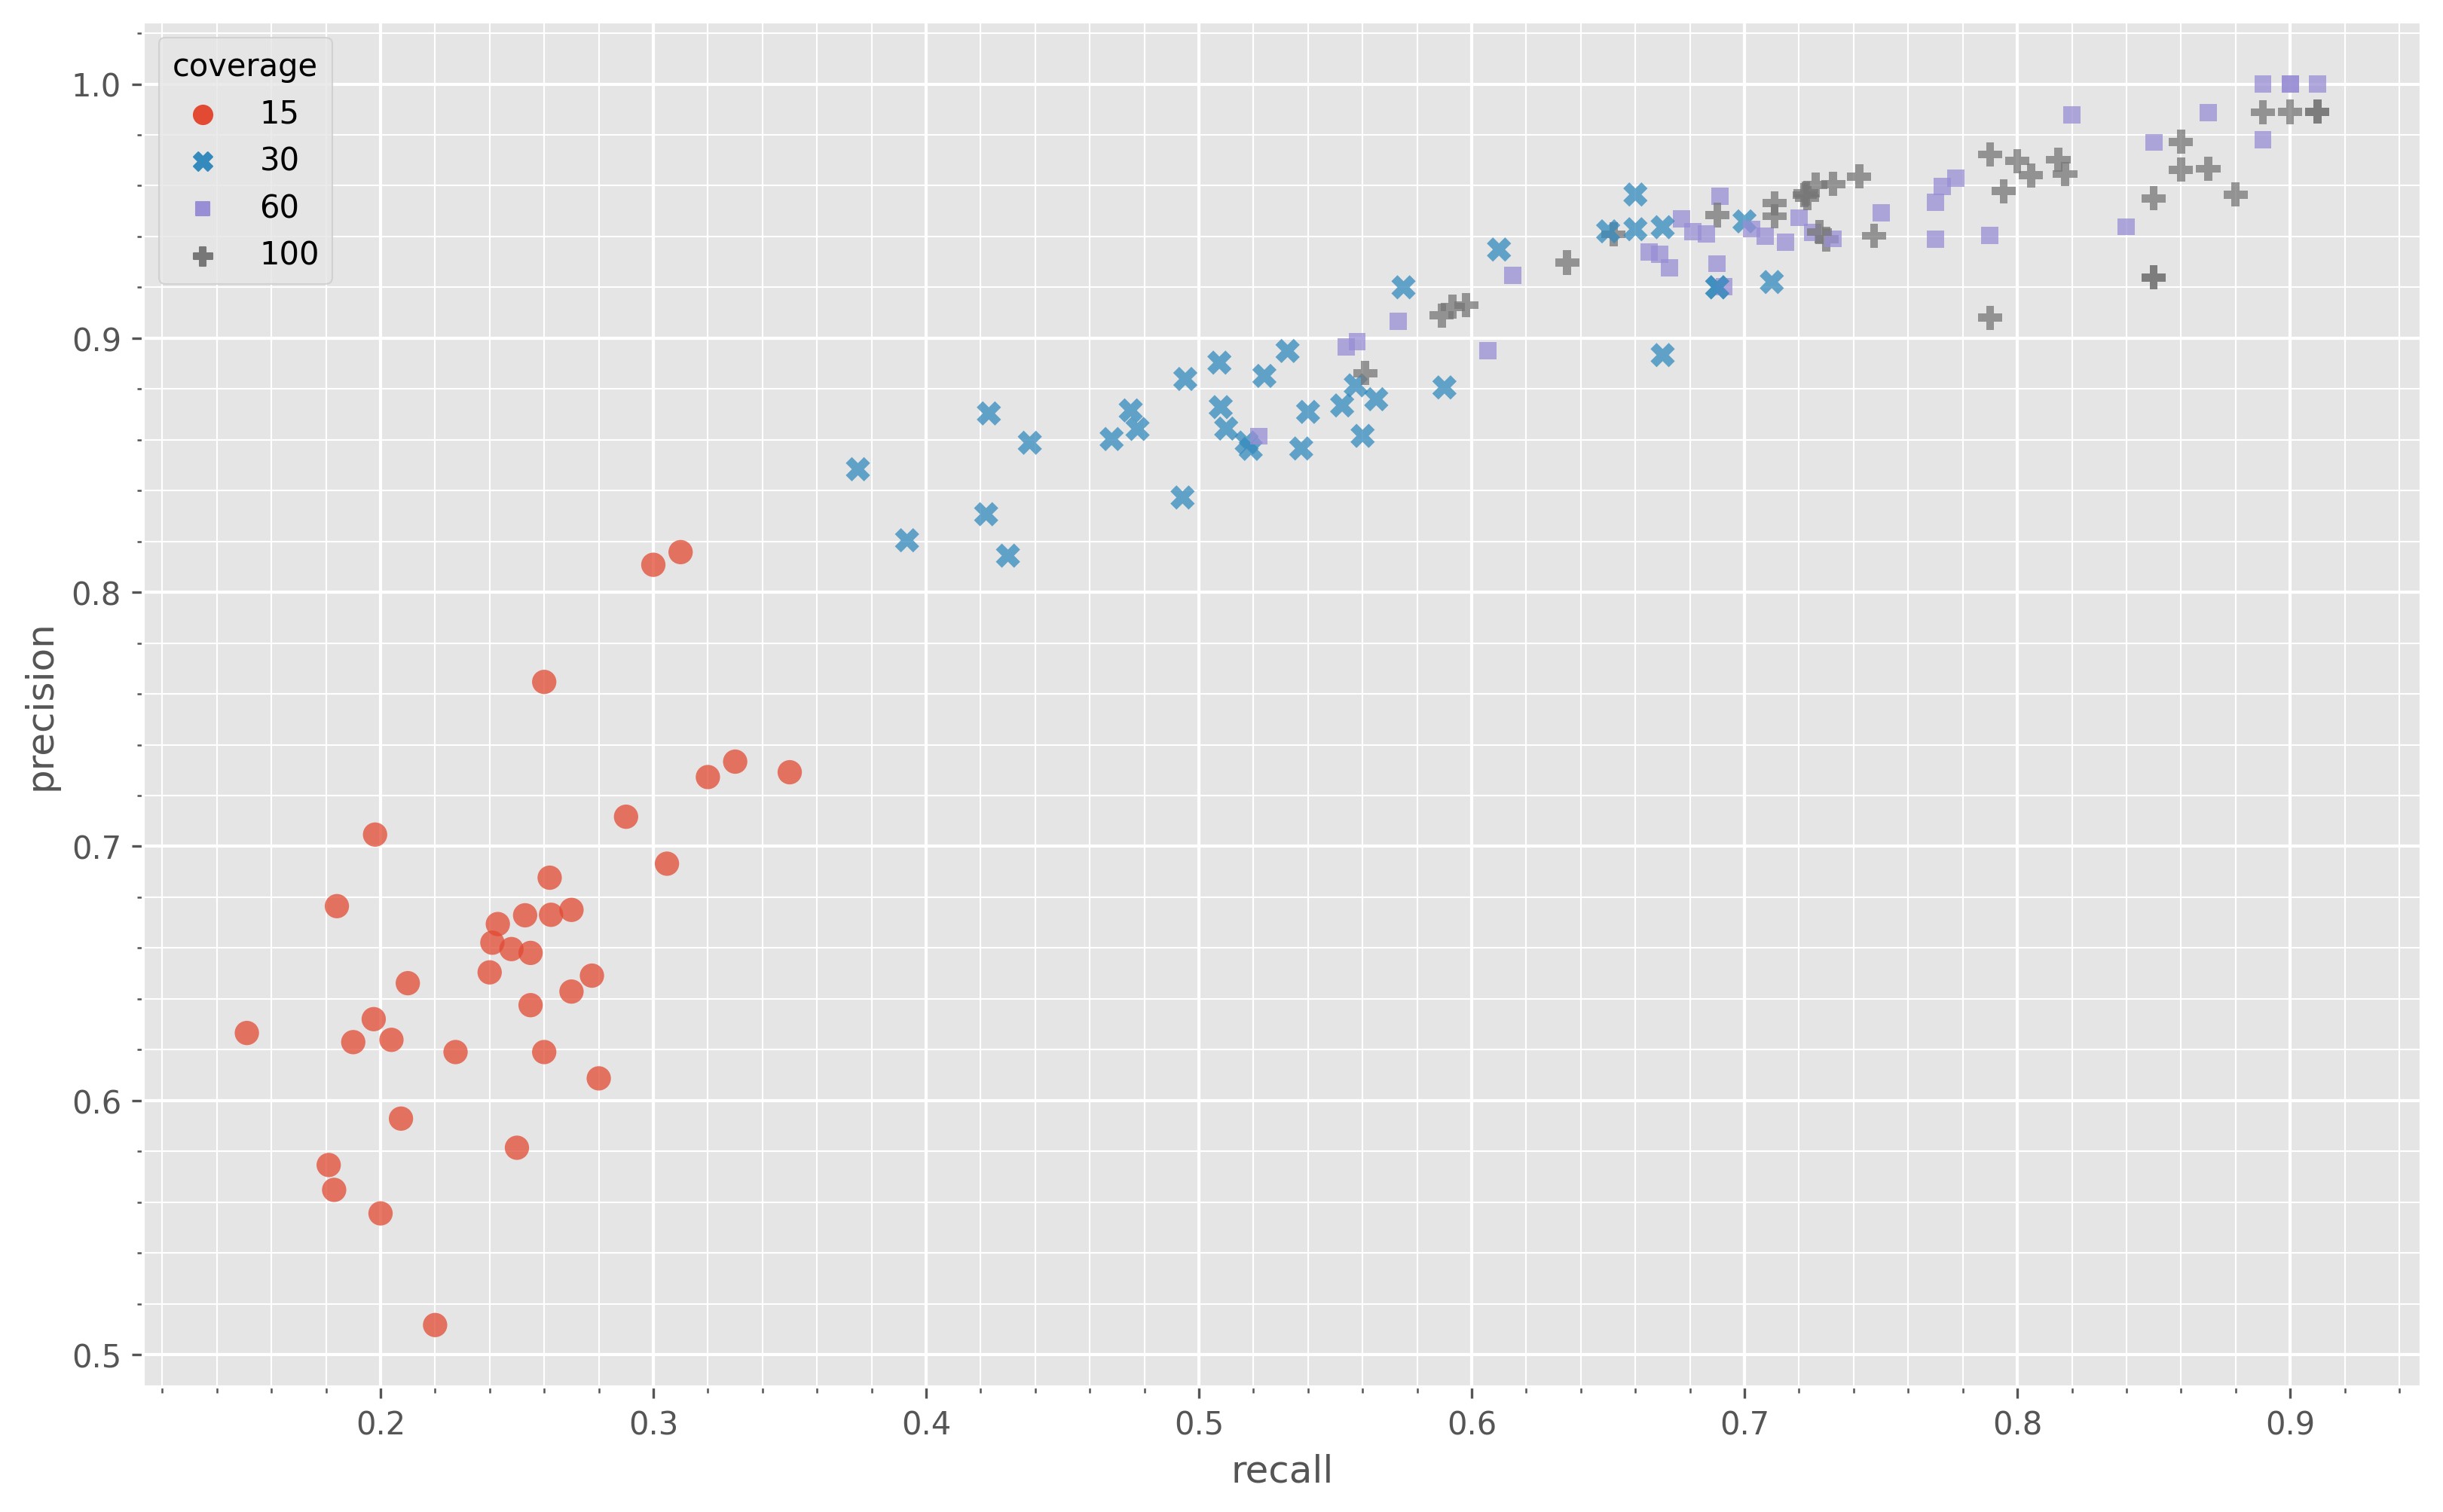
\includegraphics[width=1\linewidth]{Chapter1/Figs/denovo_precrec_covg.png}
        \centering
        \caption{Simulated coverage (read depth)}
        \label{fig:denovo-sims-covg}
     \end{subfigure}
     \begin{subfigure}[b]{0.475\textwidth}
         \centering
        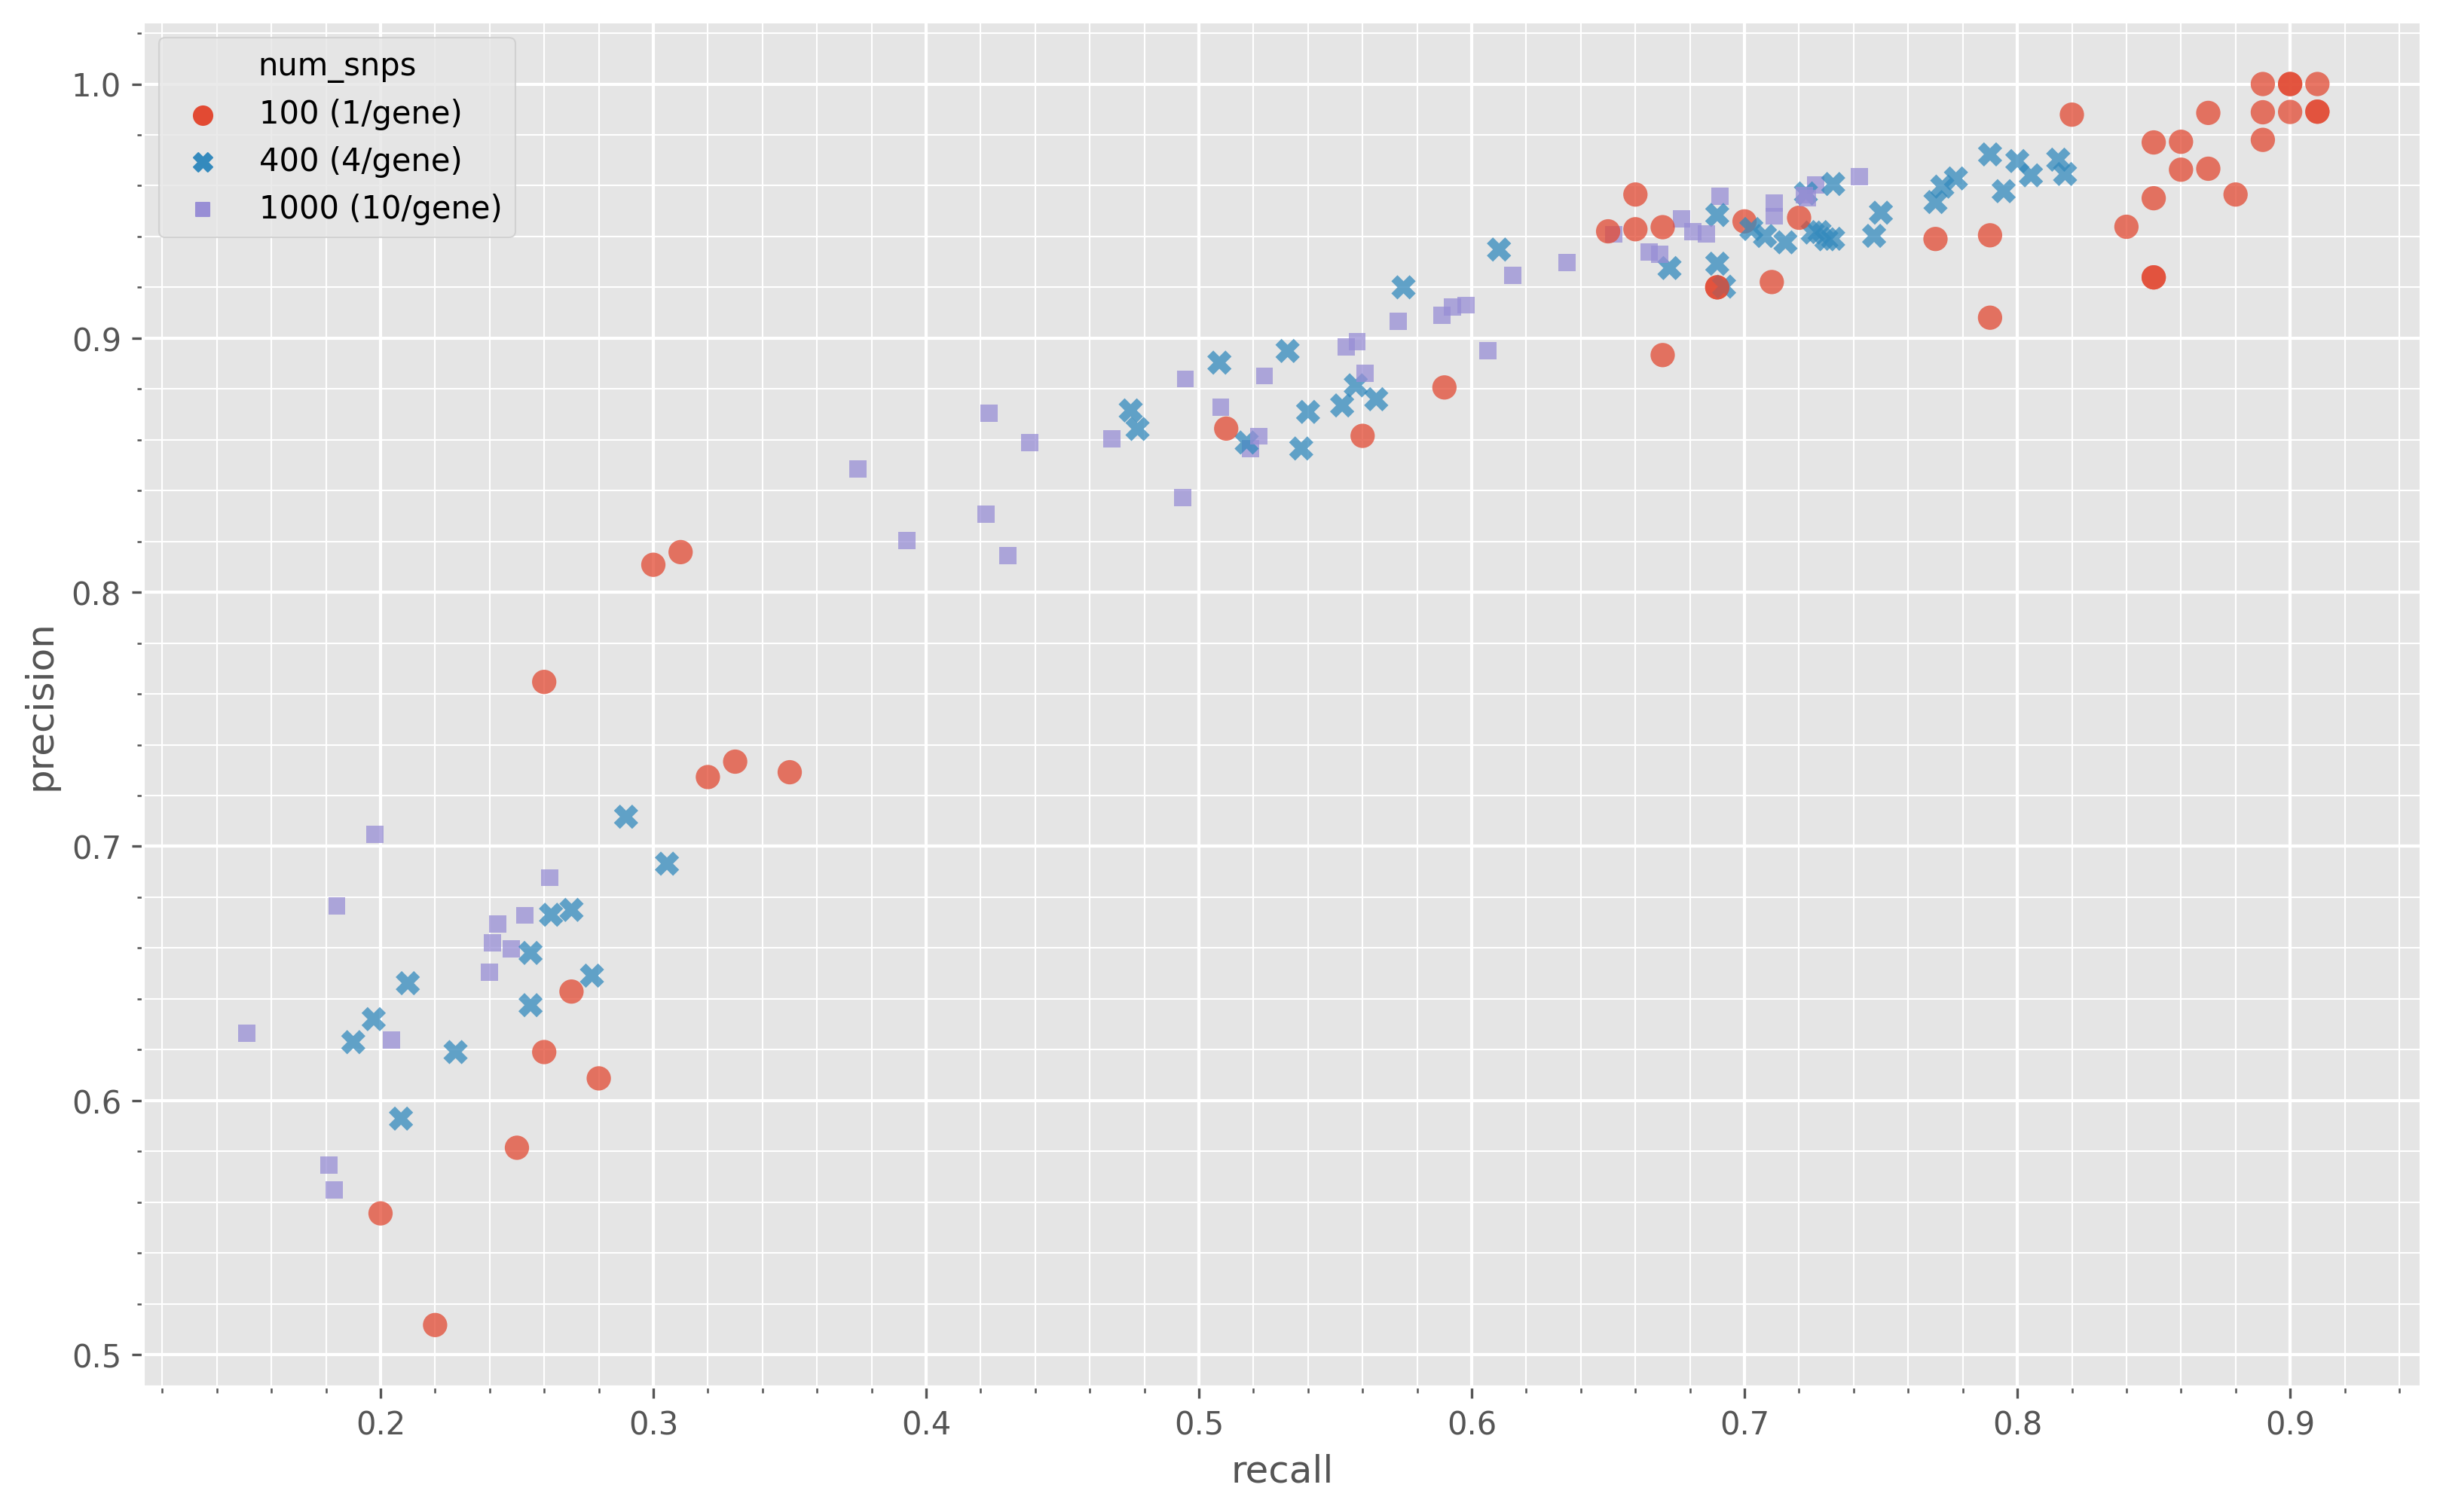
\includegraphics[width=1\linewidth]{Chapter1/Figs/denovo_precrec_num_snps.png}
         \caption{Number of SNPs simulated}
         \label{fig:denovo-sims-num-snps}
     \end{subfigure}
     \begin{subfigure}[b]{0.475\textwidth}
        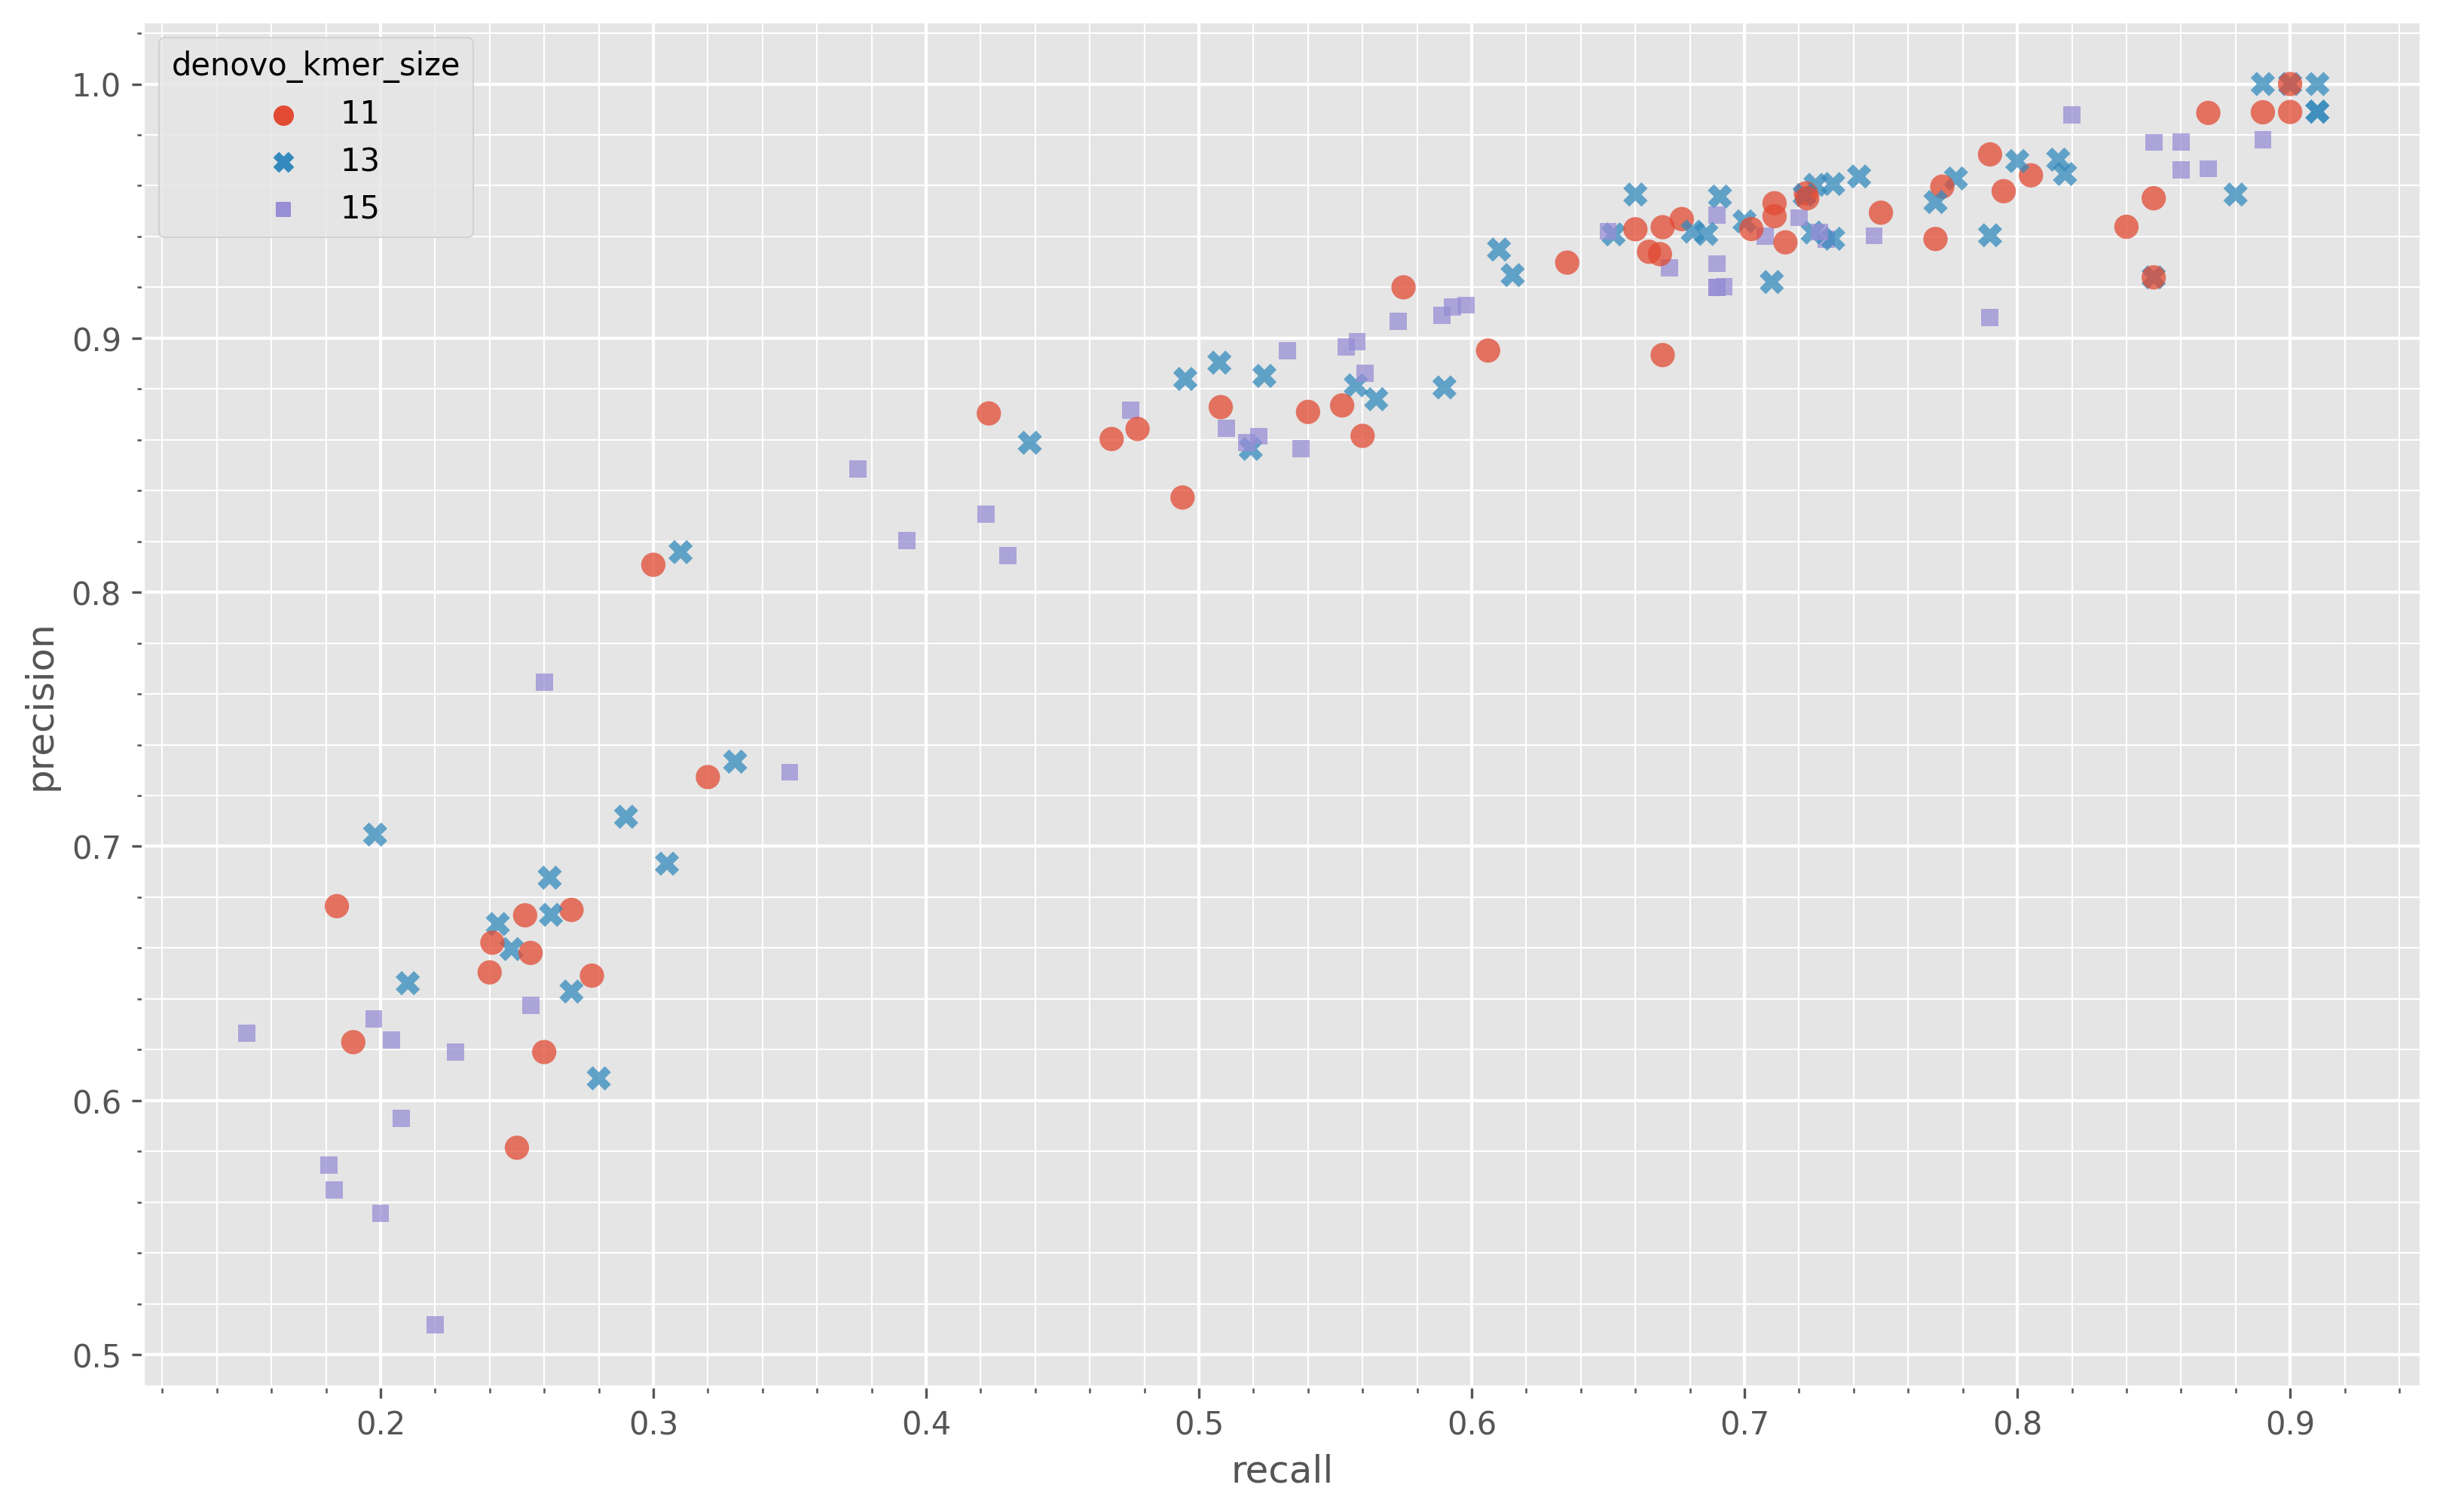
\includegraphics[width=1\linewidth]{Chapter1/Figs/denovo_precrec_kmer.png}
        \centering
        \caption{\denovo{} discovery \kmer{} size}
        \label{fig:denovo-sims-kmer-size}
     \end{subfigure}
     \begin{subfigure}[b]{0.475\textwidth}
         \centering
        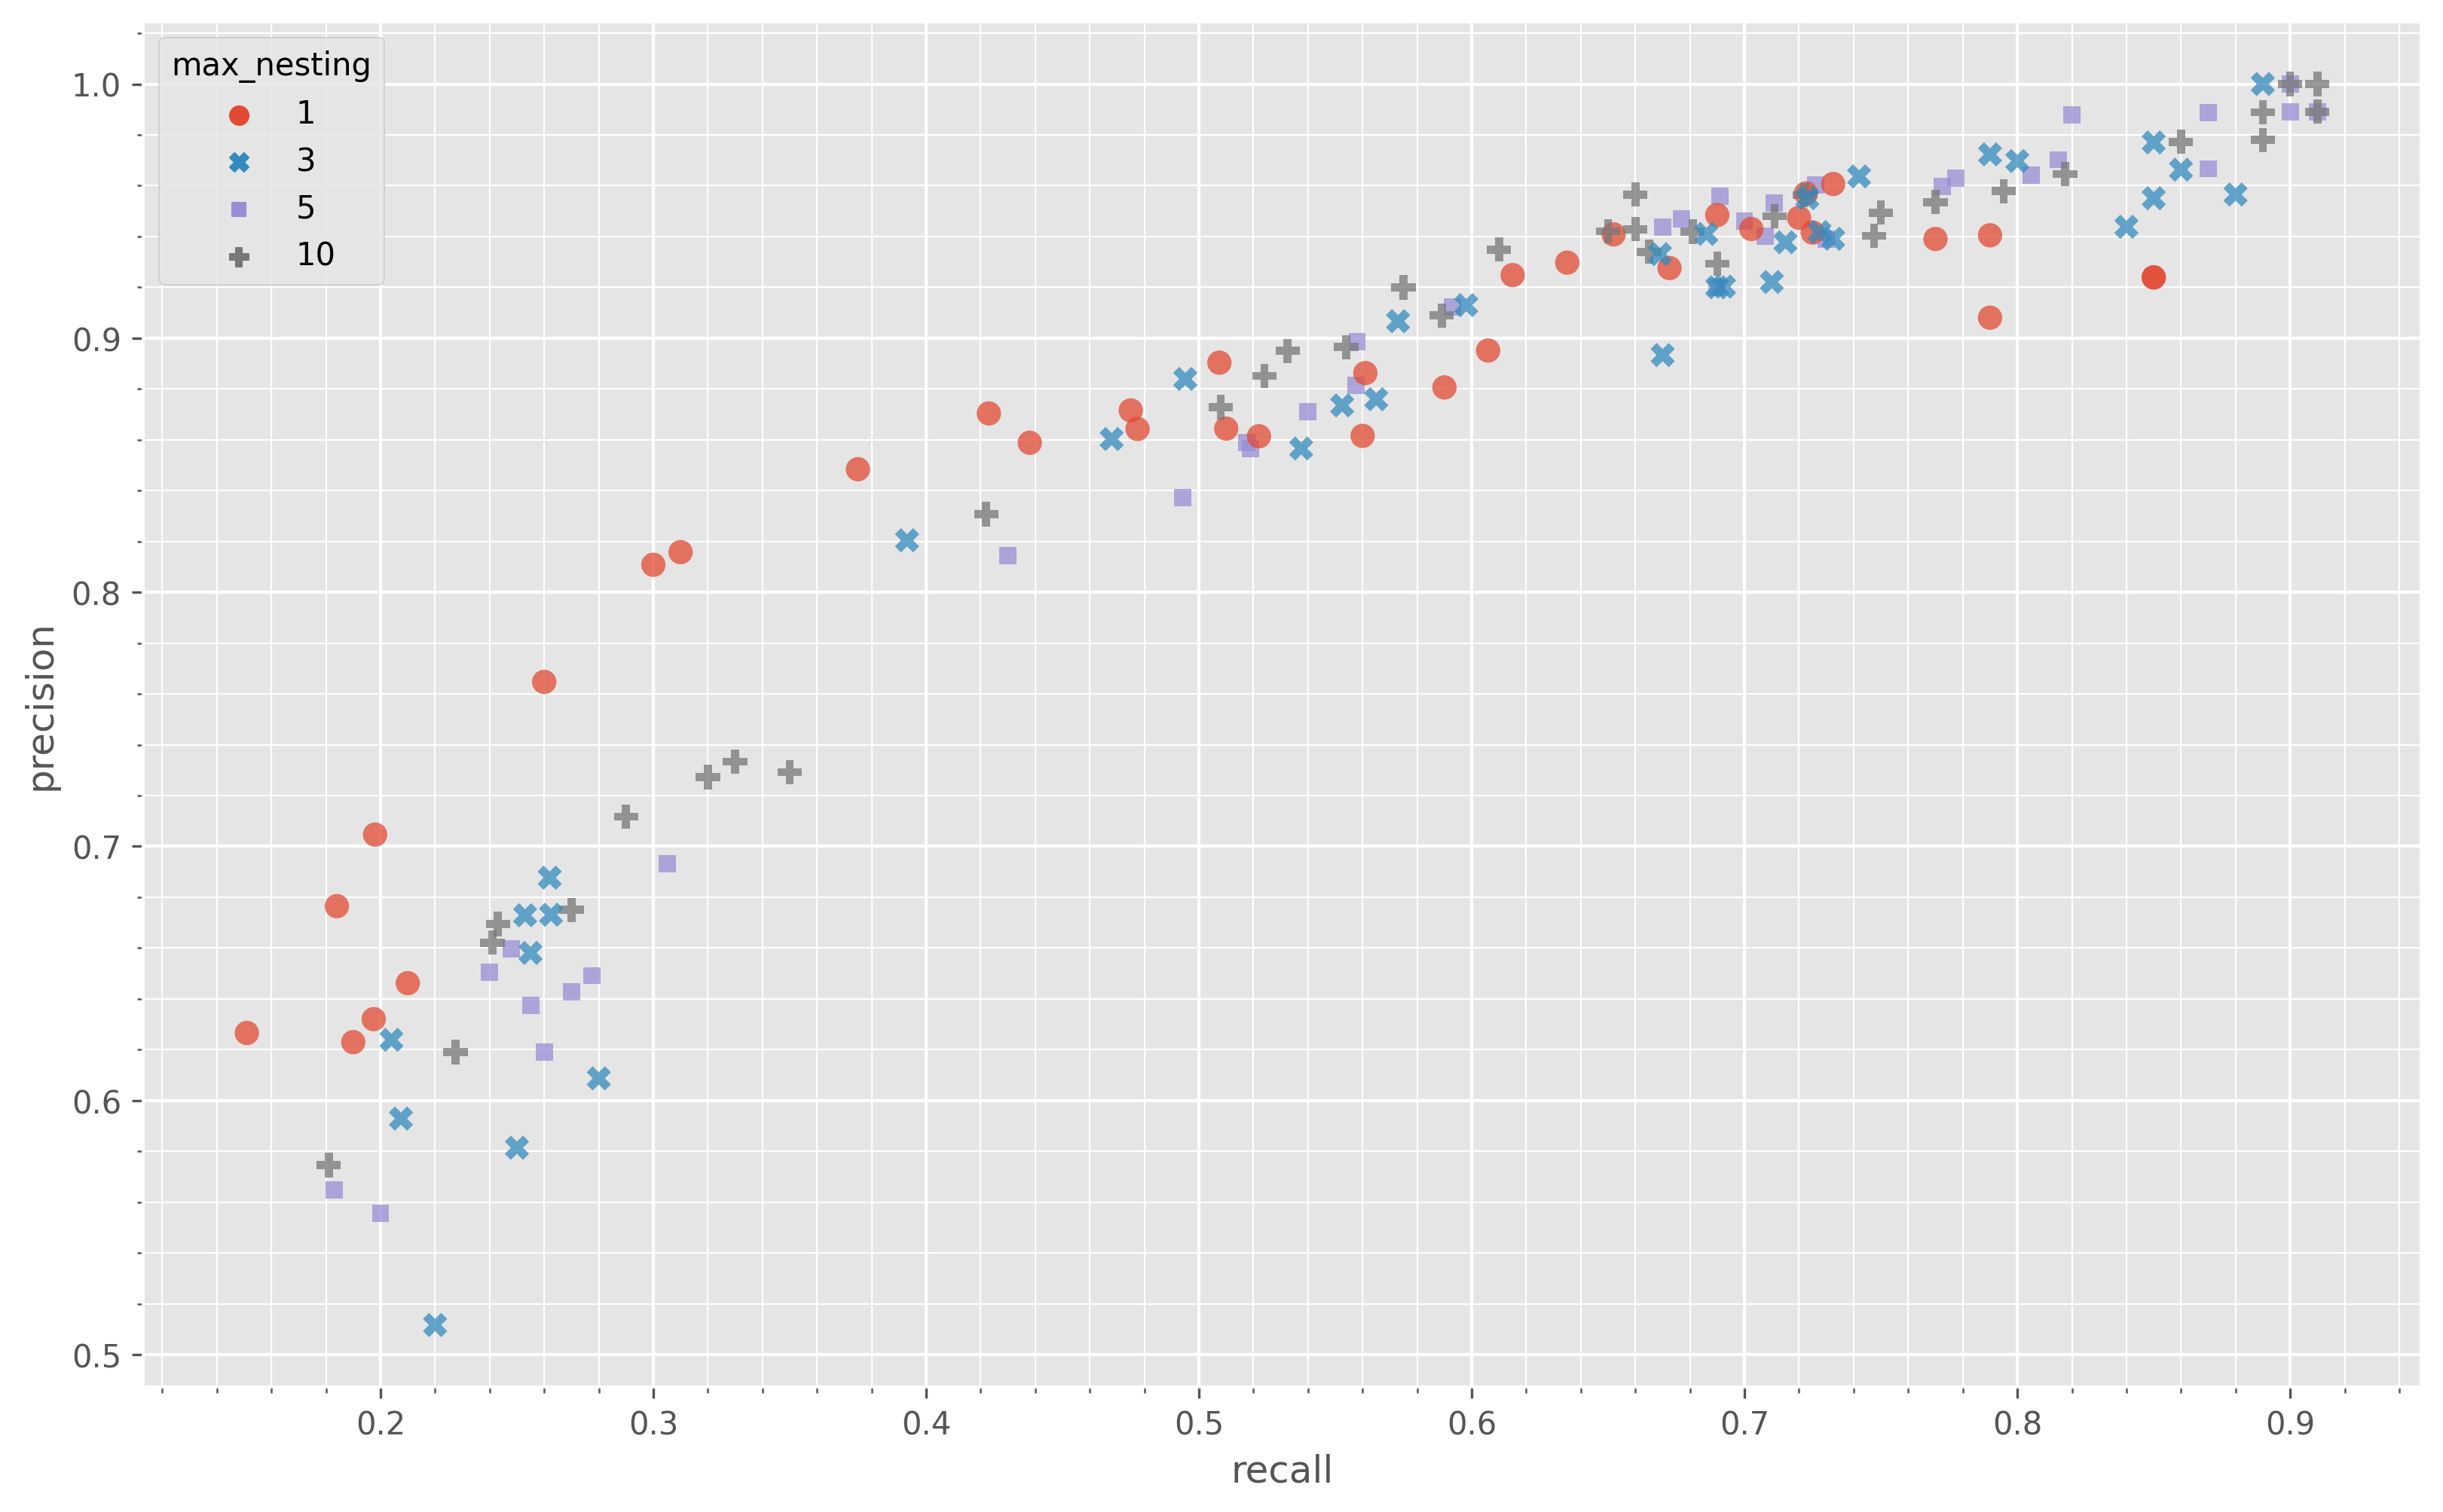
\includegraphics[width=1\linewidth]{Chapter1/Figs/denovo_precrec_nesting.png}
         \caption{\prg{} maximum nesting level}
         \label{fig:denovo-sims-nesting}
     \end{subfigure}
    \caption{Recall (x-axis) and precision (y-axis) of \denovo{} variants discovered by \pandora{} on a simulated dataset. Subplots style the points by the parameter indicated in the subtitle. Each point indicates a single run of \pandora{} with a unique combination of parameters.}
        \label{fig:denovo-sims}
\end{figure}

While not an issue for the best-performing example we have just been examining, missing loci were another common source of FNs. If \pandora{} decides a locus is not present after quasi-mapping (\autoref{sec:pandora-intro}), then obviously it is impossible for \denovo{} to discover any variants in it. We note that the vast majority of missing loci have a length less than 250 base pairs (\autoref{app:denovo-missing-lengths}).

When looking across all 144 combinations of parameters, we found that, on average, 7.8\% of variants are near the ends of loci and 2.8\% are in absent loci (\autoref{fig:denovo-errors}). 

\begin{figure}
    \centering
    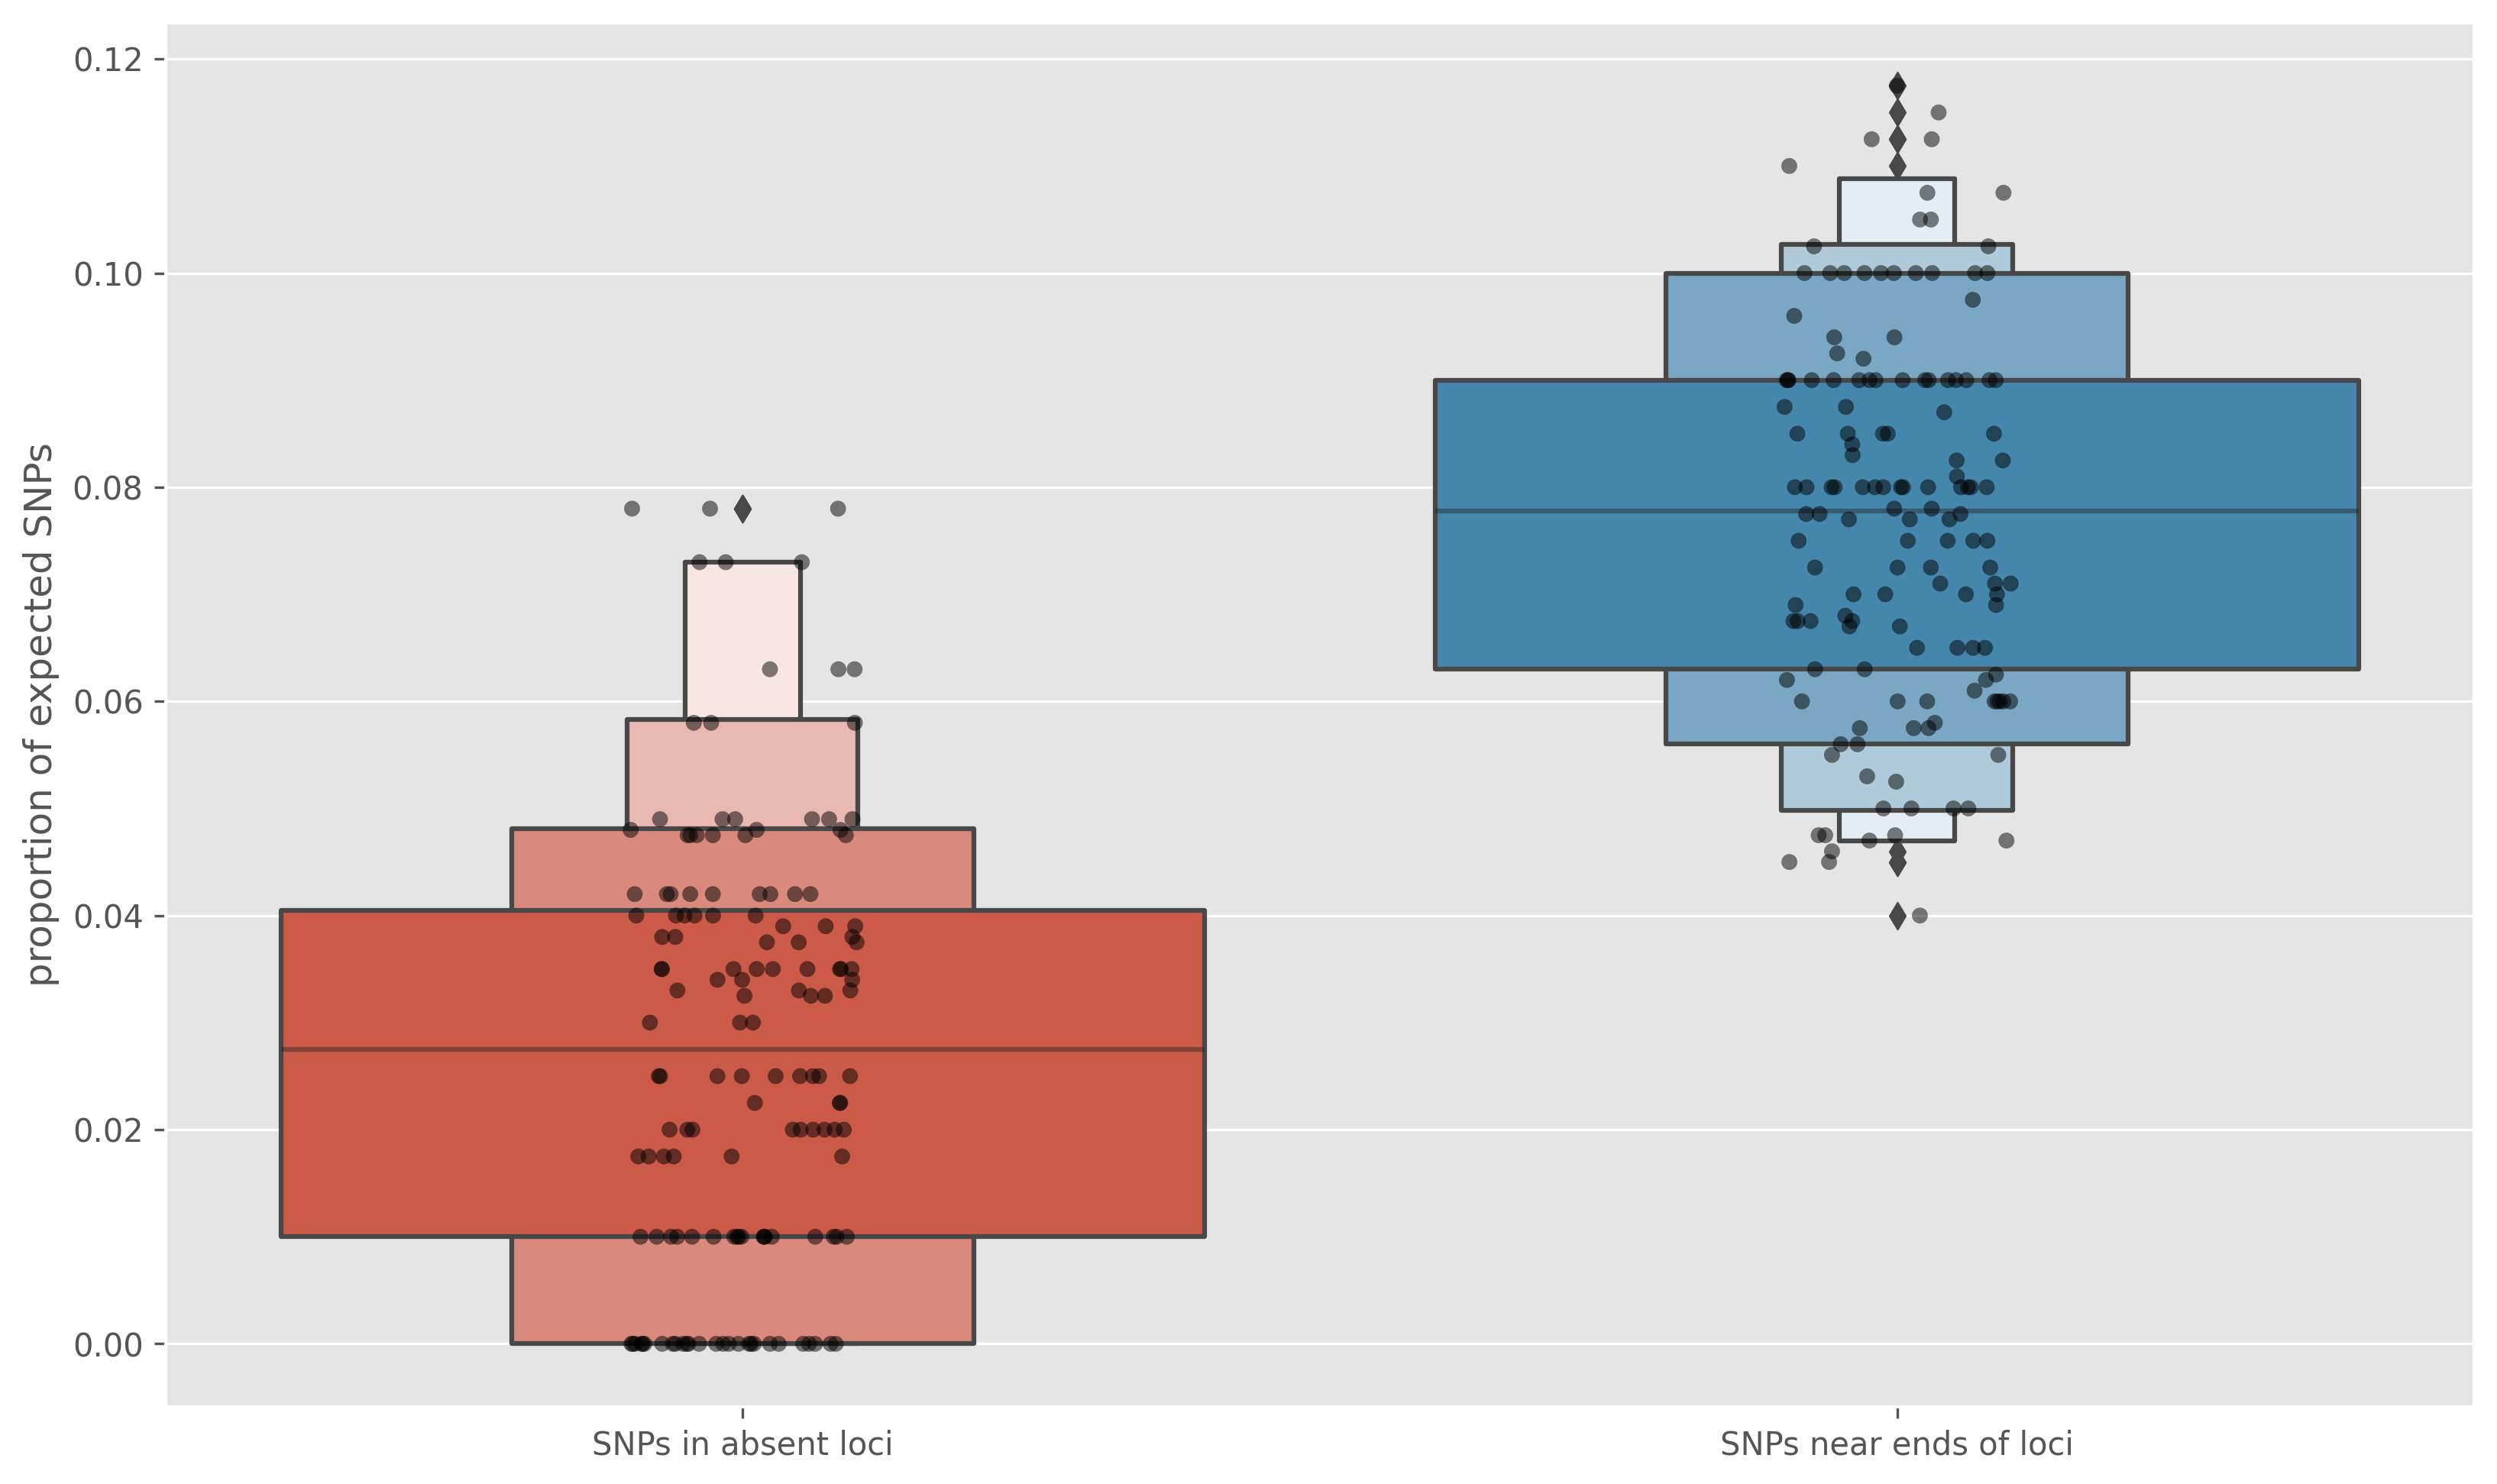
\includegraphics[width=0.9\textwidth]{Chapter1/Figs/denovo_errors.png}
    \caption{The proportion of simulated SNPs that are not detectable by \denovo{} variant discovery (y-axis). The red box represents SNPs that occur in loci designated as absent by \pandora{}. The blue box depicts the SNPs that occur within $2k-1$ positions of the start or end of a locus. Each point indicates a single run of \pandora{} with a unique combination of parameters.}
    \label{fig:denovo-errors}
\end{figure}

\noindent
The parameters that we can directly control with respect to \denovo{} discovery within \pandora{} are the \prg{} maximum nesting level and the \denovo{} \kmer{} size. \autoref{fig:denovo-sims} shows no clear optimal for either of these options. However, when taking the median precision and recall values across all data points (\autoref{tab:denovo-summary}), a maximum nesting level of 5 and \denovo{} \kmer{} size of 13 seem the best choice.

\begin{table}
\centering
\begin{tabular}{@{}lll@{}}
\toprule
          & Max. nesting & \denovo{} \kmer{} size \\ \midrule
Precision & 0.934 (10)   & 0.937 (13)                                               \\
Recall    & 0.674 (5)    & 0.671 (13)                                               \\ \bottomrule
\end{tabular}
\caption{The median precision and recall for all parameter combinations, grouping by the maximum \prg{} nesting level or the \denovo{} \kmer{} size used for variant discovery in \pandora{}. The values in parentheses indicate the parameter value that leads to the specified precision or recall.}
\label{tab:denovo-summary}
\end{table}

For the final analysis of the simulation data, we look at how the precision and recall change with an increasing genotype confidence threshold. We select the data point with the optimal maximum nesting level (5) and \denovo{} \kmer{} size (13), along with the 4 SNPs per gene, as this is within the range expected for an \ecoli{} genome. In addition, we include the data points for \pandora{} with no \denovo{} discovery. Next, starting at zero and increasing by 10 until 700, we filter out any variant with a genotype confidence score below the current threshold. The purpose of this analysis is to illustrate what the cost on recall is for requiring more confident variant calls at different read depths and the impact of including \denovo{} variant discovery in \pandora{}. 

\autoref{fig:denovo-sims-roc} shows the same relationship we saw earlier: coverage has a significant impact on precision and recall. Most importantly though, it shows that the inclusion of \denovo{} discovery is vital. As shown by the lower-left inset, the best recall achievable for this set of parameters \emph{without} variant discovery is 1.0\%. This is compared to a maximum of 81.5\% when using \denovo{} discovery. Focusing on the 100x coverage data point with \denovo{} discovery, the best recall (81.5\%) leads to a precision of 97.0\%, but the cost of increasing precision to 99\% is a drop in recall to 25\%. 

\begin{figure}
    \centering
    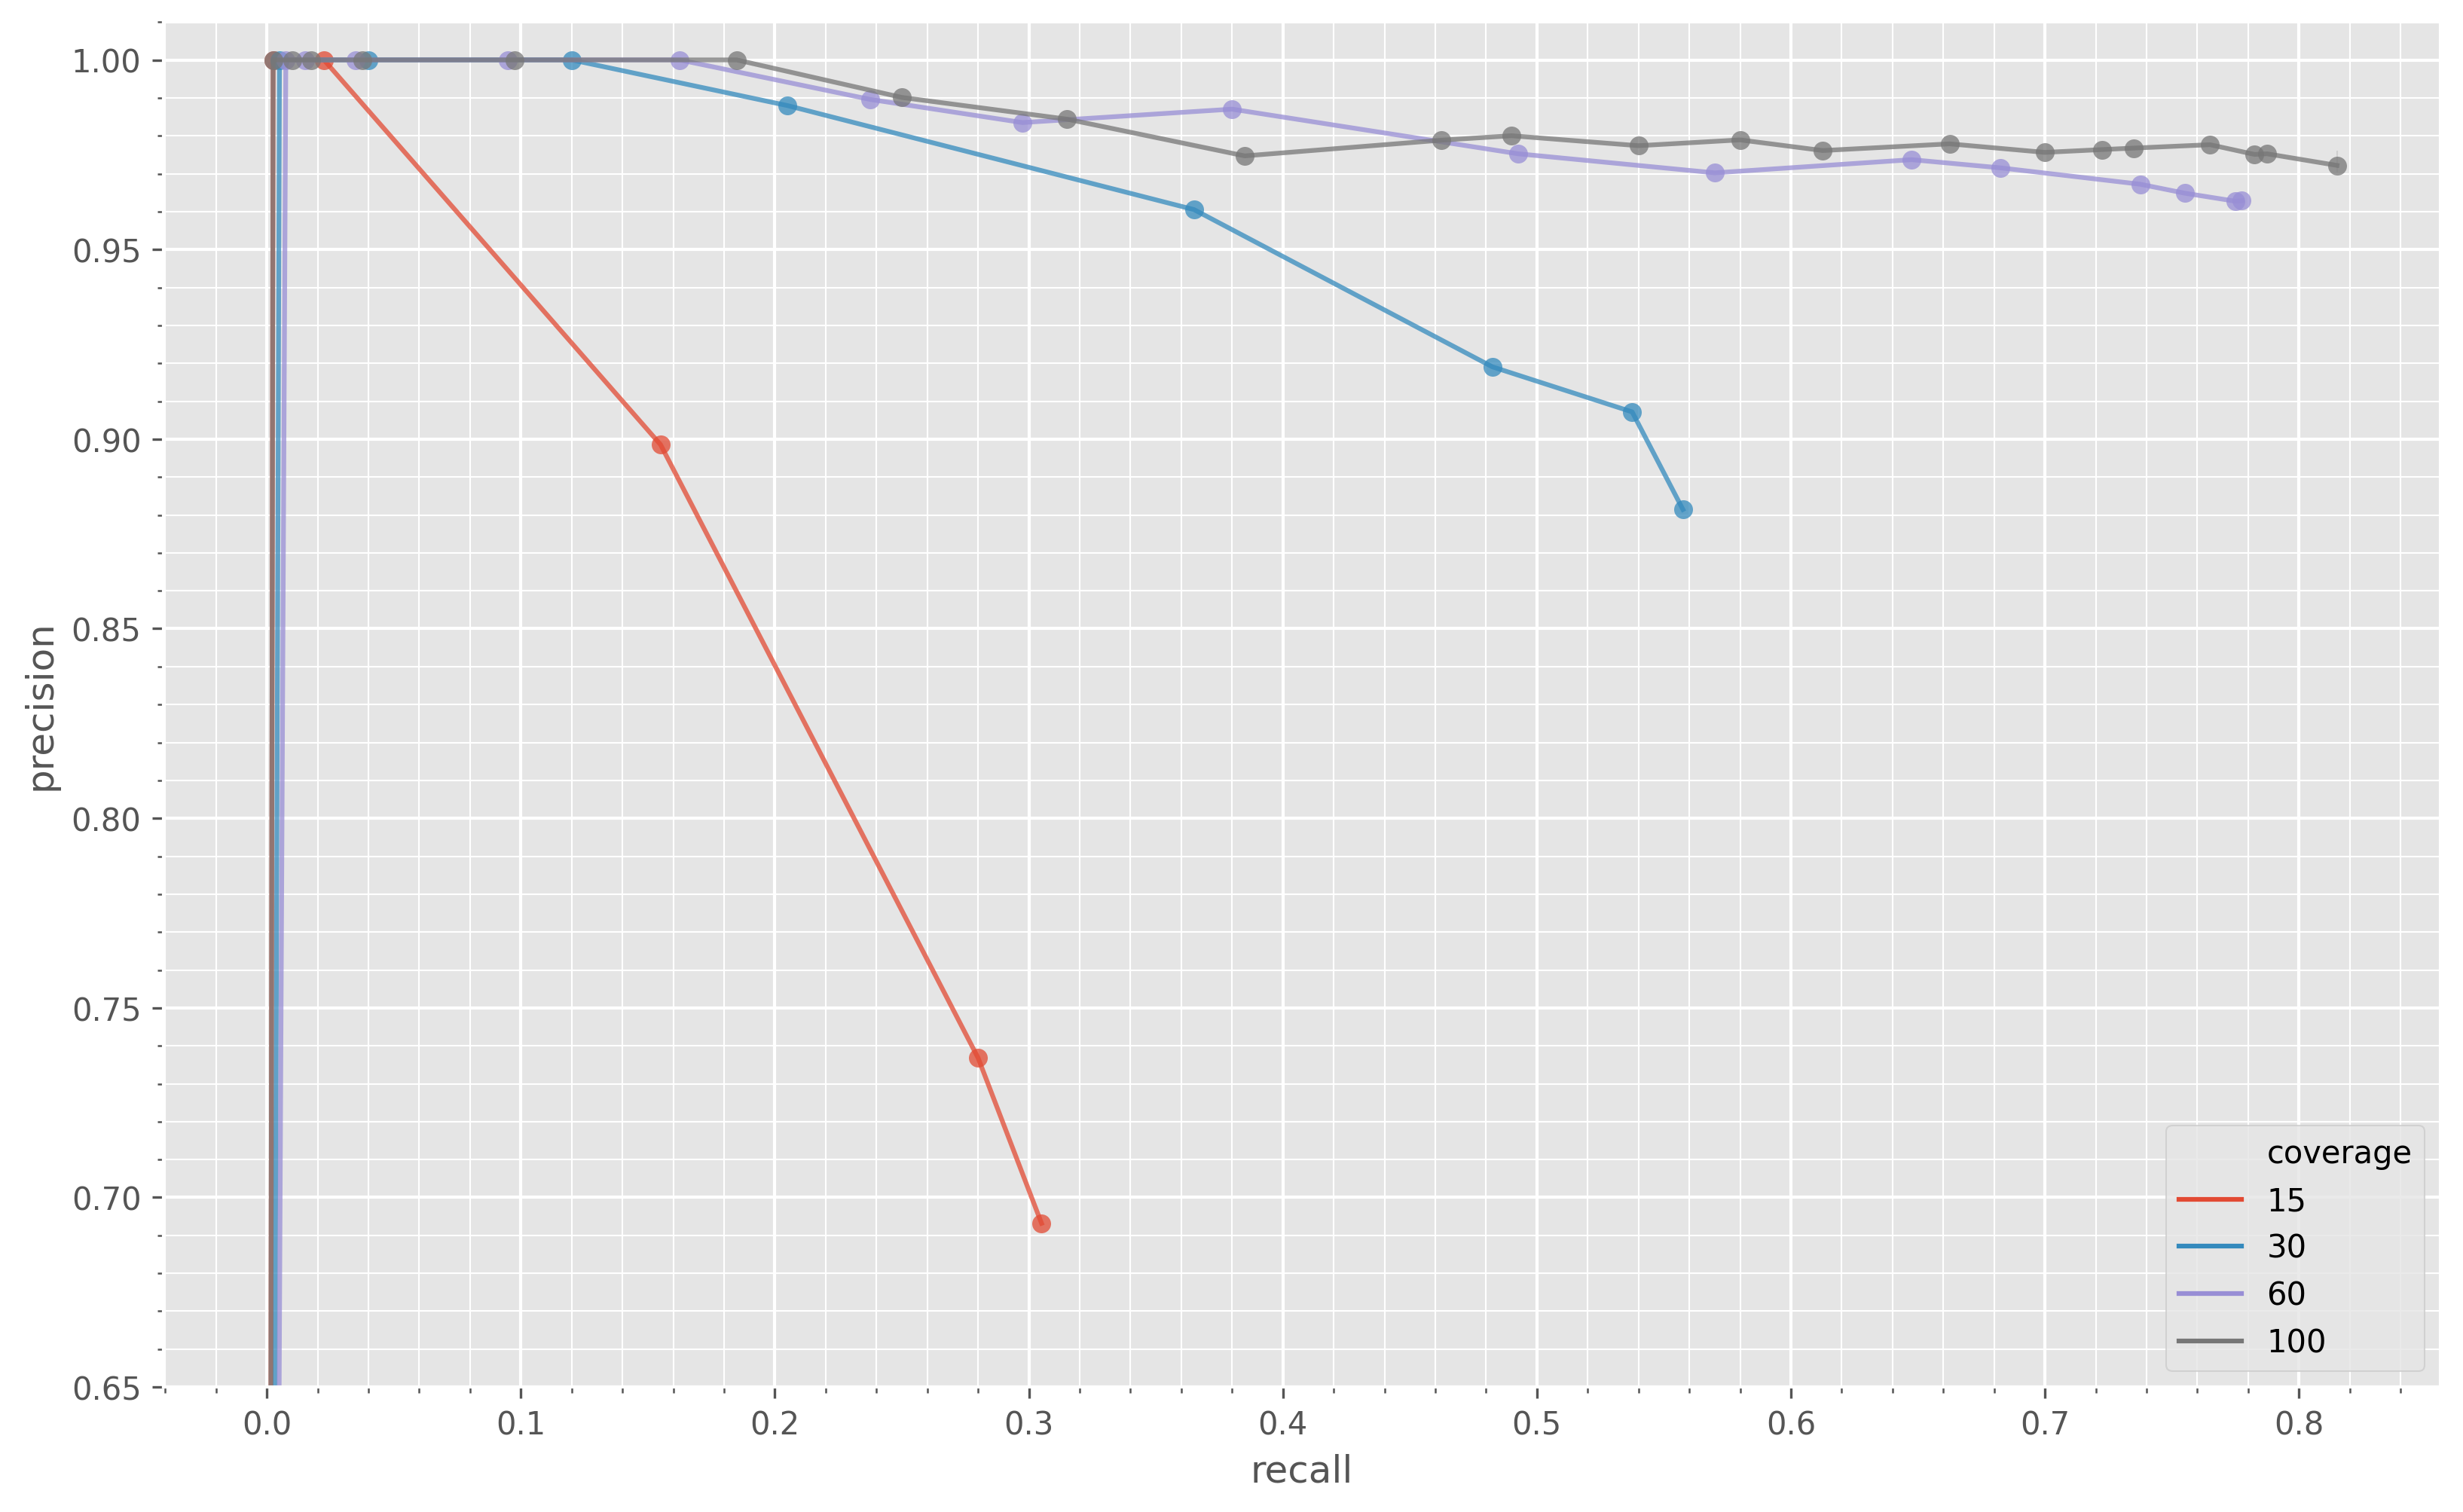
\includegraphics[width=0.9\textwidth]{Chapter1/Figs/denovo-sims-roc.png}
    \caption{Precision-recall curve for increasing genotype confidence score thresholds. The curves are coloured by read depth (coverage) and styled by whether or not \denovo{} variant discovery was used. Each marker/point is a different genotype confidence threshold, starting with 0 as the right-most value and increasing as the line moves towards the (top) left. The inset window in the lower-left of the figure shows the performance of \pandora{} without \denovo{} discovery. The inset on the right gives more granularity of precision for the higher-coverage data points.}
    \label{fig:denovo-sims-roc}
\end{figure}

\subsection{Summary}

In summary, we have shown that the addition of the \denovo{} variant discovery method outlined in \autoref{sec:denovo-method} gives \pandora{} the ability to find many variants not present its \panrg{}. Using simulated data, we find a \kmer{} size of 13 gives slightly better recall than 11 or 15, but that the sample read depth has the largest impact on our ability to discover novel variants.

We have also shown that on average, approximately 10.5\% of (simulated) SNPs are not detectable based on their membership in either loci \pandora{} does not detect, or within $2k-1$ positions of the end of a locus.

% ==================================================================
\section{Empirical data}
\label{sec:denovo-empirical}

Having shown, for simulated data, that the \denovo{} variant discovery method indeed alleviates the major limitation of \pandora{}, we now turn our attention to evaluating its performance on empirical data. However, rather than the single-sample (\pandora{} \vrb{map}) approach we used for genotyping in \autoref{sec:denovo-sims}, we evaluate \pandora{}'s multi-sample comparison protocol - \compare{}.

The inference of variation within a collection of samples is one of the unique aspects of \pandora{}. As detailed in \autoref{sec:pandora-compare}, the \vrb{compare} routine of \pandora{} genotypes multiple samples against a \panrg{} simultaneously, with the aim of representing variation in the most succinct manner possible (see \autoref{fig:var-representation}). It does this by selecting a maximum likelihood path that best approximates the samples under investigation.

Evaluating the variant calls from such a graph-based method is by no means trivial. In this section we aim to compare the variant calls made by \pandora{} against those made by single-reference (linear) methods for both Illumina and \ont{} data. As such, in addition to the variant calling evaluation, we outline a novel approach to compare variants produced from a graph-based reference with those from a linear reference.

In keeping with the focus of this chapter, we will also assess the utility of \denovo{} variant discovery within \pandora{}. While we have shown its benefit on simulated data, the \panrg{} used did not contain many of the simulated SNPs. However, we expect many of the SNPs in real data to also be present in a \panrg{} built from a pan-genome of diverse samples. 

\textit{Note: all work in this section is described in full in \cite{pandora}. See \autoref{sec:denovo-acknowledge} for a detailed description of what work was completed by myself.}

\subsection{Dataset}
\label{sec:denovo-empirical-data}

\subsubsection{Samples}
The empirical data we use for this evaluation is a diverse set of 20 \ecoli{} samples from four different phylogroups. Each sample was sequenced on both \ont{} and Illumina platforms and have high quality assemblies available. The sequencing reads for each technology were subsampled to 100x read depth.

\subsubsection{References}
The \panrg{} we use as the reference for \pandora{} was constructed from a combination of \ecoli{} genes and intergenic regions. 23,054 gene MSAs from 350 RefSeq genomes were obtained from the panX database \cite{panx}, while 14,374 intergenic region MSAs from 228 ST131 genomes were collected from \cite{thorpe2018}. \prg{}s were constructed for each locus using \makeprg{} and then all were combined into a single \panrg{} file and indexed with \pandora{}.

As single-reference variant callers cannot use a \panrg{}, we selected 24 reference genomes from five major phylogroups; one phylogroup is not contained within the sample set. These refeerences were selected to be spread across each phylogroup, ensuring some were close to our samples and some not. By calling variants for each sample with respect to each reference genome, we can directly view the impact of reference selection on the results of standard variant callers.

\subsection{Variant calling}

\subsubsection{Graph-based: Pandora}
To produce a multi-sample VCF file of variants for \pandora{} we follow a somewhat similar approach to \autoref{sec:denovo-sims-methods}, with some important differences. Rather than adding all \denovo{} variants for a single sample to the original \panrg{} we instead add the novel variants for \emph{all} samples to the original \panrg{}. In the end, we have an updated \panrg{} which contains all novel variants for all samples under comparison. We then perform multi-sample genotyping with this updated \panrg{} using \compare{}. This entire process is completed separately for Illumina and \ont{} data.

\subsubsection{Linear-based}
We compare the Illumina variant calls from \pandora{} against those from \vrb{samtools} \cite{samtools2009} and Snippy (\url{https://github.com/tseemann/snippy}) (which is a wrapper around Freebayes \cite{Garrison2012}). The \ont{} variant callers we evaluate against are Medaka (\url{https://github.com/nanoporetech/medaka}) and Nanopolish \cite{Loman2015}. Each variant caller is run on all 20 samples with all 24 reference genomes. 

\noindent
In total, we produce 480 VCFs for each linear variant caller and 20 (one per sample) for \pandora{}.

\subsection{Evaluation}
\label{sec:denovo-empirical-eval}

A direct comparison of the VCF files produced by \pandora{} and the single-reference tools is not possible due to coordinate incompatibilities. As such, we use a probe-based method, akin to that in \autoref{sec:denovo-sims-eval}, for assessing the variant calls. 

The first step in this evaluation is the generation of a pan-genome SNP truth set. \autoref{app:pangenome-snp-truth} details the construction of this truth set, resulting in 618,305 SNPs we expect to find amongst the 20 samples.

There are two measures of recall in a pan-genome (see \autoref{app:pangenome-snp-truth}), but of interest to this section is the average allelic recall (AvgAR). Briefly, AvgAR  is the average recall of all pan-genome variants. For example, say we have three genomes with 2 pan-genome variants $P1$ and $P2$ between them. $P1$ has the alleles A, G, and T across the three genomes and $P2$ has alleles C and T. If we find the $P1$ alleles A and T, we have a $P1$ recall of 0.66 (2/3) and if we only find $P2$ alleles C, we have a $P2$ recall of 0.5 (1/2). Therefore, in this example, we have an AvgAR of $\frac{0.66+0.5}{2}=0.58$.

To calculate AvgAR (recall) for tool-reference pair, we perform the following: i) apply the variant calls for each sample to the reference sequence the calls were made with respect to (giving 20 mutated sequences); ii) we map all truth set probes to these mutated reference sequence with \vrb{bwa mem}; iii) we classify a mapping as TP if the aligned sequences match. We then count, for each pan-genome variant, what proportion of its alleles have a TP mapping and calculate AvgAR accordingly. In the end, we have an AvgAR value for each variant caller and reference sequence combination - i.e., 24 AvgAR values for each caller.

We determine precision in a somewhat similar manner. First, we create probes for each variant in a given VCF, with 150bp flanking sequence taken from the VCF reference sequence. Second, we map each probe to the sample's assembly sequence. Third, we filter out poor quality mappings or mappings to low quality regions of the assembly. Fourth, each mapping's precision is classified as a continuous score - rather than a binary true or false positive - by dividing the number of matching bases (ignoring the flanking sequences), divided by the length of the alignment. For example, if the called allele is ATG and it maps to a sequence ATTG, the precision score is 0.75. Finally, we calculate the precision as the sum of precision scores, divided by the number of evaluated calls.

\subsection{Effect of different \ont{} basecalling models}
\label{sec:denovo-methylation}

Previous work from Wick \etal{} has shown that for Enterobacteriaceae the majority of \ont{} sequencing errors are related to Dcm methylation sites \cite{wick2019}. In version 3.2.1 of \guppy{} (the ONT-provided basecalling software) a new \emph{methylation-aware} model was made available. However, this new model is considerably slower to basecall reads than the default model. As \ecoli{} is a member of this family, we set out to test a subset of 4 samples from our dataset to see whether a methylation-aware model indeed has a noticeable impact on the precision and recall from \pandora{} - with and without \denovo{} variant dicsovery.

We basecall the raw data for 4 samples from our dataset with both the default and methylation-aware models from \guppy{} version 3.4.5. Precision and recall (AvgAR) are calculated as per \autoref{sec:denovo-empirical-eval} and presented in \autoref{fig:denovo-methylation}. The precision-recall curves represent increasing genotype confidence filtering; the top-right of each curve is no filtering, and as the genotype confidence requirement is gradually increased, we reduce the error rate (increase precision) at the loss of recall. Two important observations from \autoref{fig:denovo-methylation} are that the use of a methylation-aware model increases both precision \emph{and} recall, and the use of \denovo{} discovery increases recall at the cost of precision. \autoref{tab:denovo-methylation} shows the precision and recall values for the unfiltered results (i.e., the top-right of each curve in \autoref{fig:denovo-methylation}). From this, we see that without \denovo{} variant discovery, using a methylation-aware model would allow us to recover 894.7 variants in 10000 - 3.3 more than with the default model; likewise, we would expect to make 0.5 errors per 1000 variants. Using \denovo{} variant discovery, the methylation-aware model allows us to disocver 906.3 variants in 1000 - 4.8 more than the default model and 11.6 more than methylation-aware without \denovo{} discovery. In terms of errors, using a methylation-aware model leads to 3.7 less error per 1000 variants with novel variant discovery enabled, however, it does 0.41 more errors per 1000 variants than without novel variant discovery. 

\begin{figure}
    \centering
    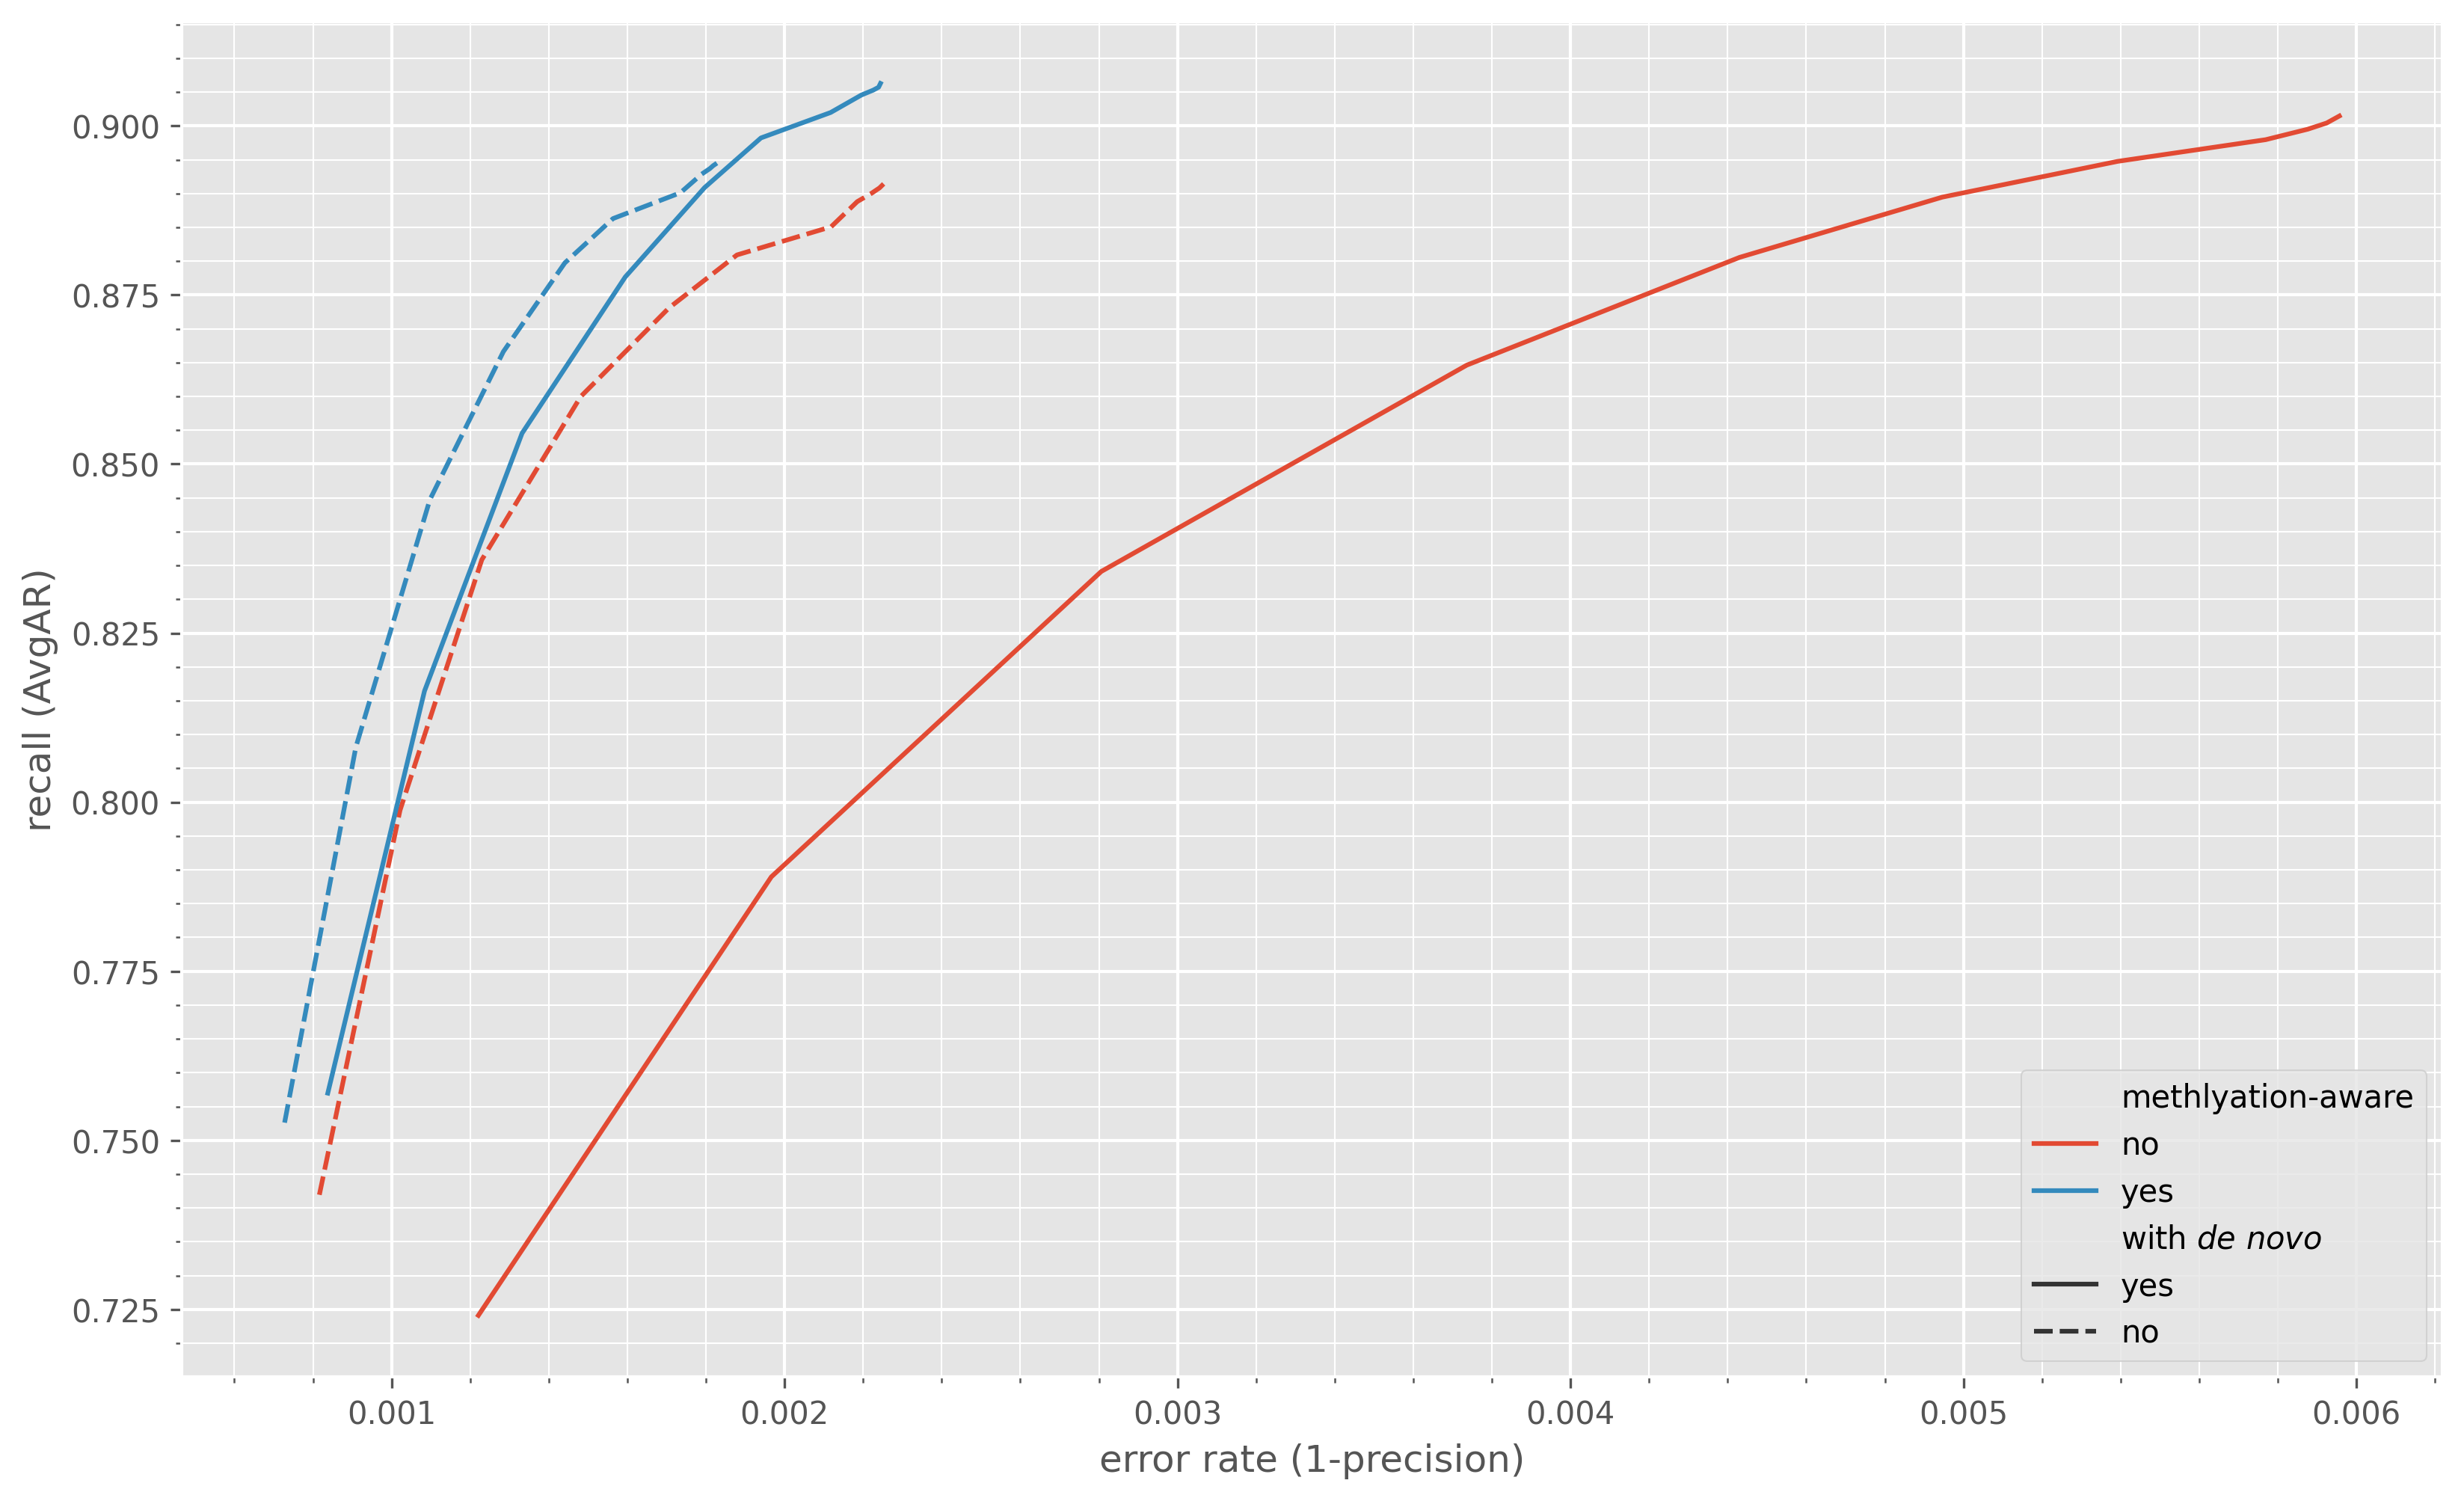
\includegraphics[width=0.9\textwidth]{Chapter1/Figs/pandora_basecaller_roc.png}
    \caption{Effect of \ont{} methylation-aware basecalling model on \pandora{} \denovo{} variant discovery. The lines show the recall (average alleleic recall; y-axis) and error rate ($1-$precision; x-axis) of \pandora{} with increasing genotype confidence score thresholds with (solid line) and without (dashed line) \denovo{} variant discovery. The red line shows samples that were basecalled with the default \guppy{} model, with those in blue being basecalled with a methylation-aware model.}
    \label{fig:denovo-methylation}
\end{figure}

\begin{table}[]
\centering
\begin{tabular}{@{}llrr@{}}
\toprule
    Methylation-aware    & with \denovo{} & Recall (AvgAR)  & Error rate ($1-$precision) \\ \midrule
\multirow{2}{*}{no}  & yes                   & 0.9015          & 0.0060                   \\
                     & no                    & 0.8914          & 0.0023                   \\
\multirow{2}{*}{yes} & yes                   & \textbf{0.9063} & 0.0022                   \\
                     & no                    & 0.8947          & \textbf{0.0018}          \\ \cmidrule(l){2-4} 
\end{tabular}
    \caption{Effect of \ont{} methylation-aware basecalling model on \pandora{} \denovo{} variant discovery (unfiltered) precision and recall.}
\label{tab:denovo-methylation}
\end{table}

\noindent
Given the dramatic improvement in precision and recall from using the methylation-aware basecalling model, we re-basecalled all data for subsequent analyses with this model.

\subsection{Performance of \pandora{} against single-reference tools}

We now compare the precision and recall of \pandora{} on Illumina and \ont{} data against to two single-reference variant callers for each technology. For the \ont{} analysis, we use the reads basecalled with the methylation-aware model (\autoref{sec:denovo-methylation}). In addition, we run \pandora{} with and without \denovo{} variant discovery in order to see the impact of the work in this chapter.

We use AvgAR as the measure of recall (see \autoref{sec:denovo-empirical-eval}) and error rate as the measure of precision ($1-$precision) and apply increasing genotype confidence thresholds to illustrate the precision-recall trade-off. 

The results of this analysis are shown in \autoref{fig:pandora-roc}. For both sequencing technologies, \pandora{} with \denovo{} variant discovery has the highest (unfiltered) recall of 85.82\% on Illumina data and 85.51\% on \ont{}. In terms of error rate, \vrb{snippy} had the lowest Illumina unfiltered value of 0.01\% (with reference CP010170.1), while \pandora{} without \denovo{} variant discovery had the lowest \ont{} unfiltered rate of 0.19\%. 

Of particular interest to the work in this chapter is the observation that, on Illumina data, \denovo{} variant discovery leads to greater recall and precision (see inset of \autoref{fig:pandora-roc-illumina}); however, on \ont{} data \denovo{} discovery only provides greater recall, at the cost of lower precision (see inset of \autoref{fig:pandora-roc-ont}). This suggests that systematic errors in \ont{} create incorrect novel alleles which are in turn deemed correct by genotyping.

The most striking result from this work though is the error rate of \pandora{} on \ont{} data, which is 12.9 times lower than \vrb{nanopolish} and 79 times lower than \vrb{medaka}. In real terms, this equates to 22 and 146 less error per 1000 variants, respectively.

Equally impressive is the improvement in recall over \vrb{snippy} using \pandora{} with variant discovery on Illumina data, leading to 47/1000 more variants being discovered. However, as noted above, this does come at the expense of a higher error rate than \vrb{snippy}.

\begin{figure}
     \begin{subfigure}[b]{0.475\textwidth}
        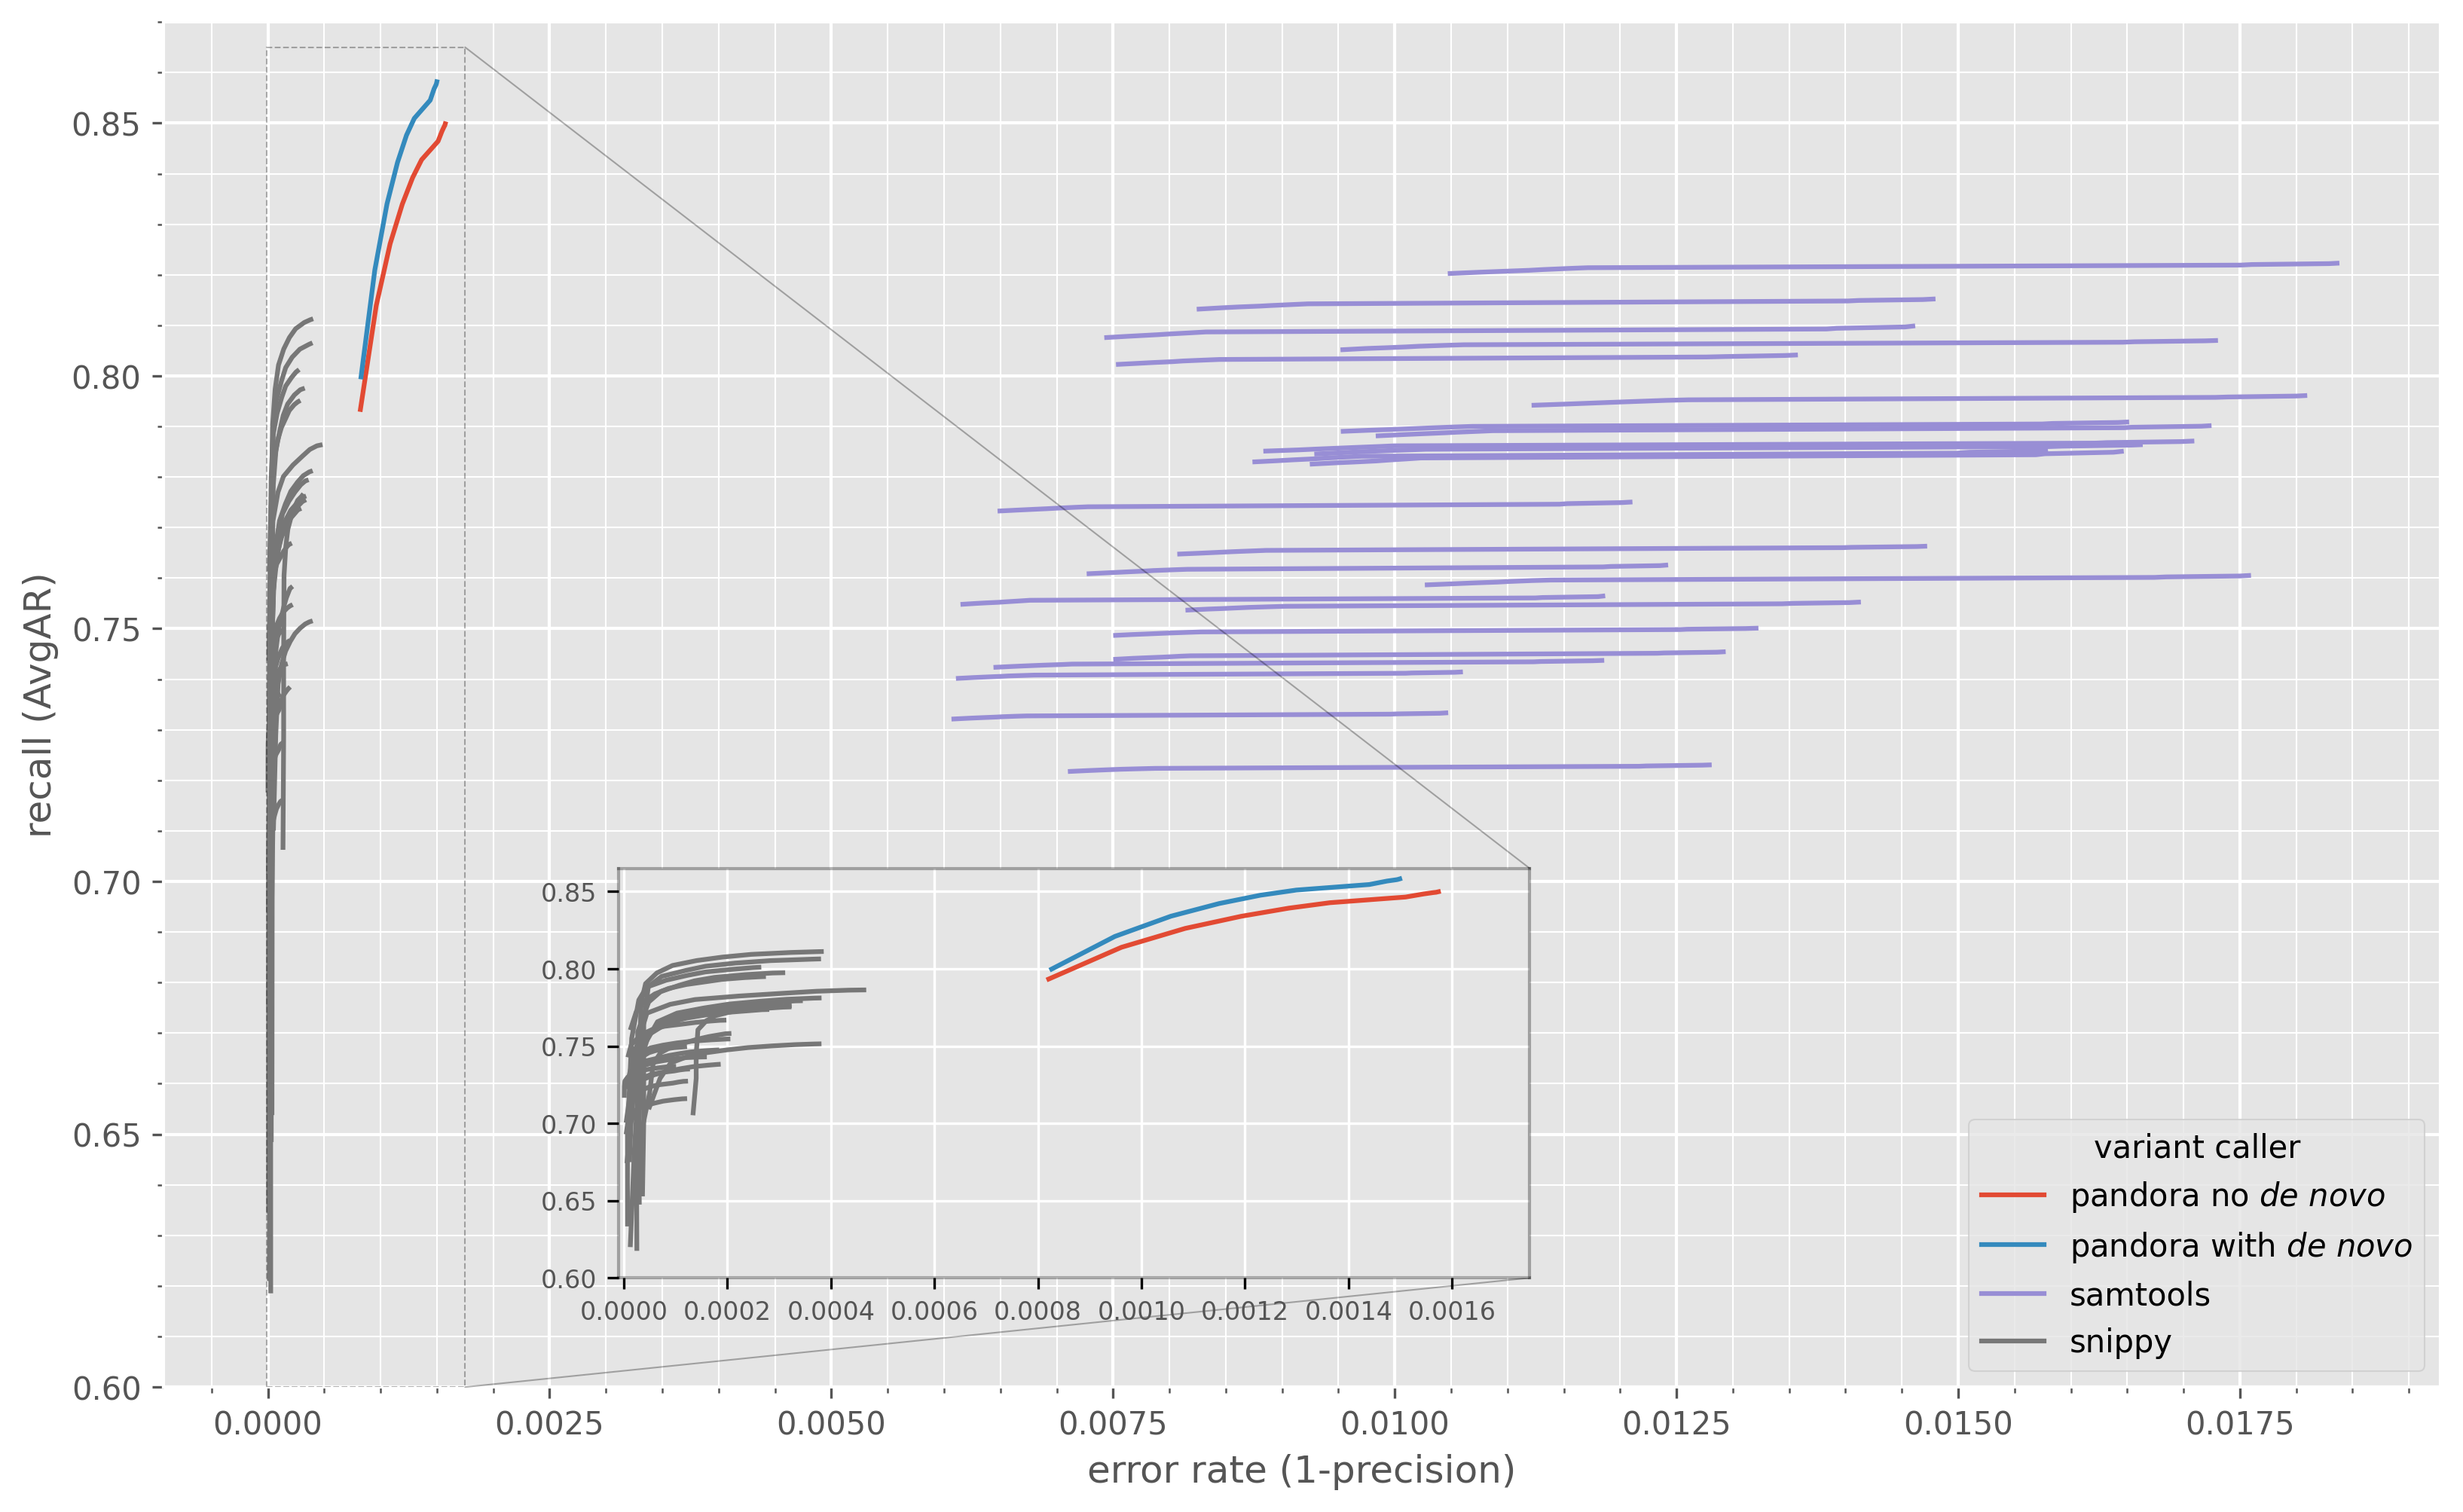
\includegraphics[width=1\linewidth]{Chapter1/Figs/illumina_roc.png}
        \centering
        \caption{Illumina}
        \label{fig:pandora-roc-illumina}
     \end{subfigure}
     \begin{subfigure}[b]{0.475\textwidth}
         \centering
        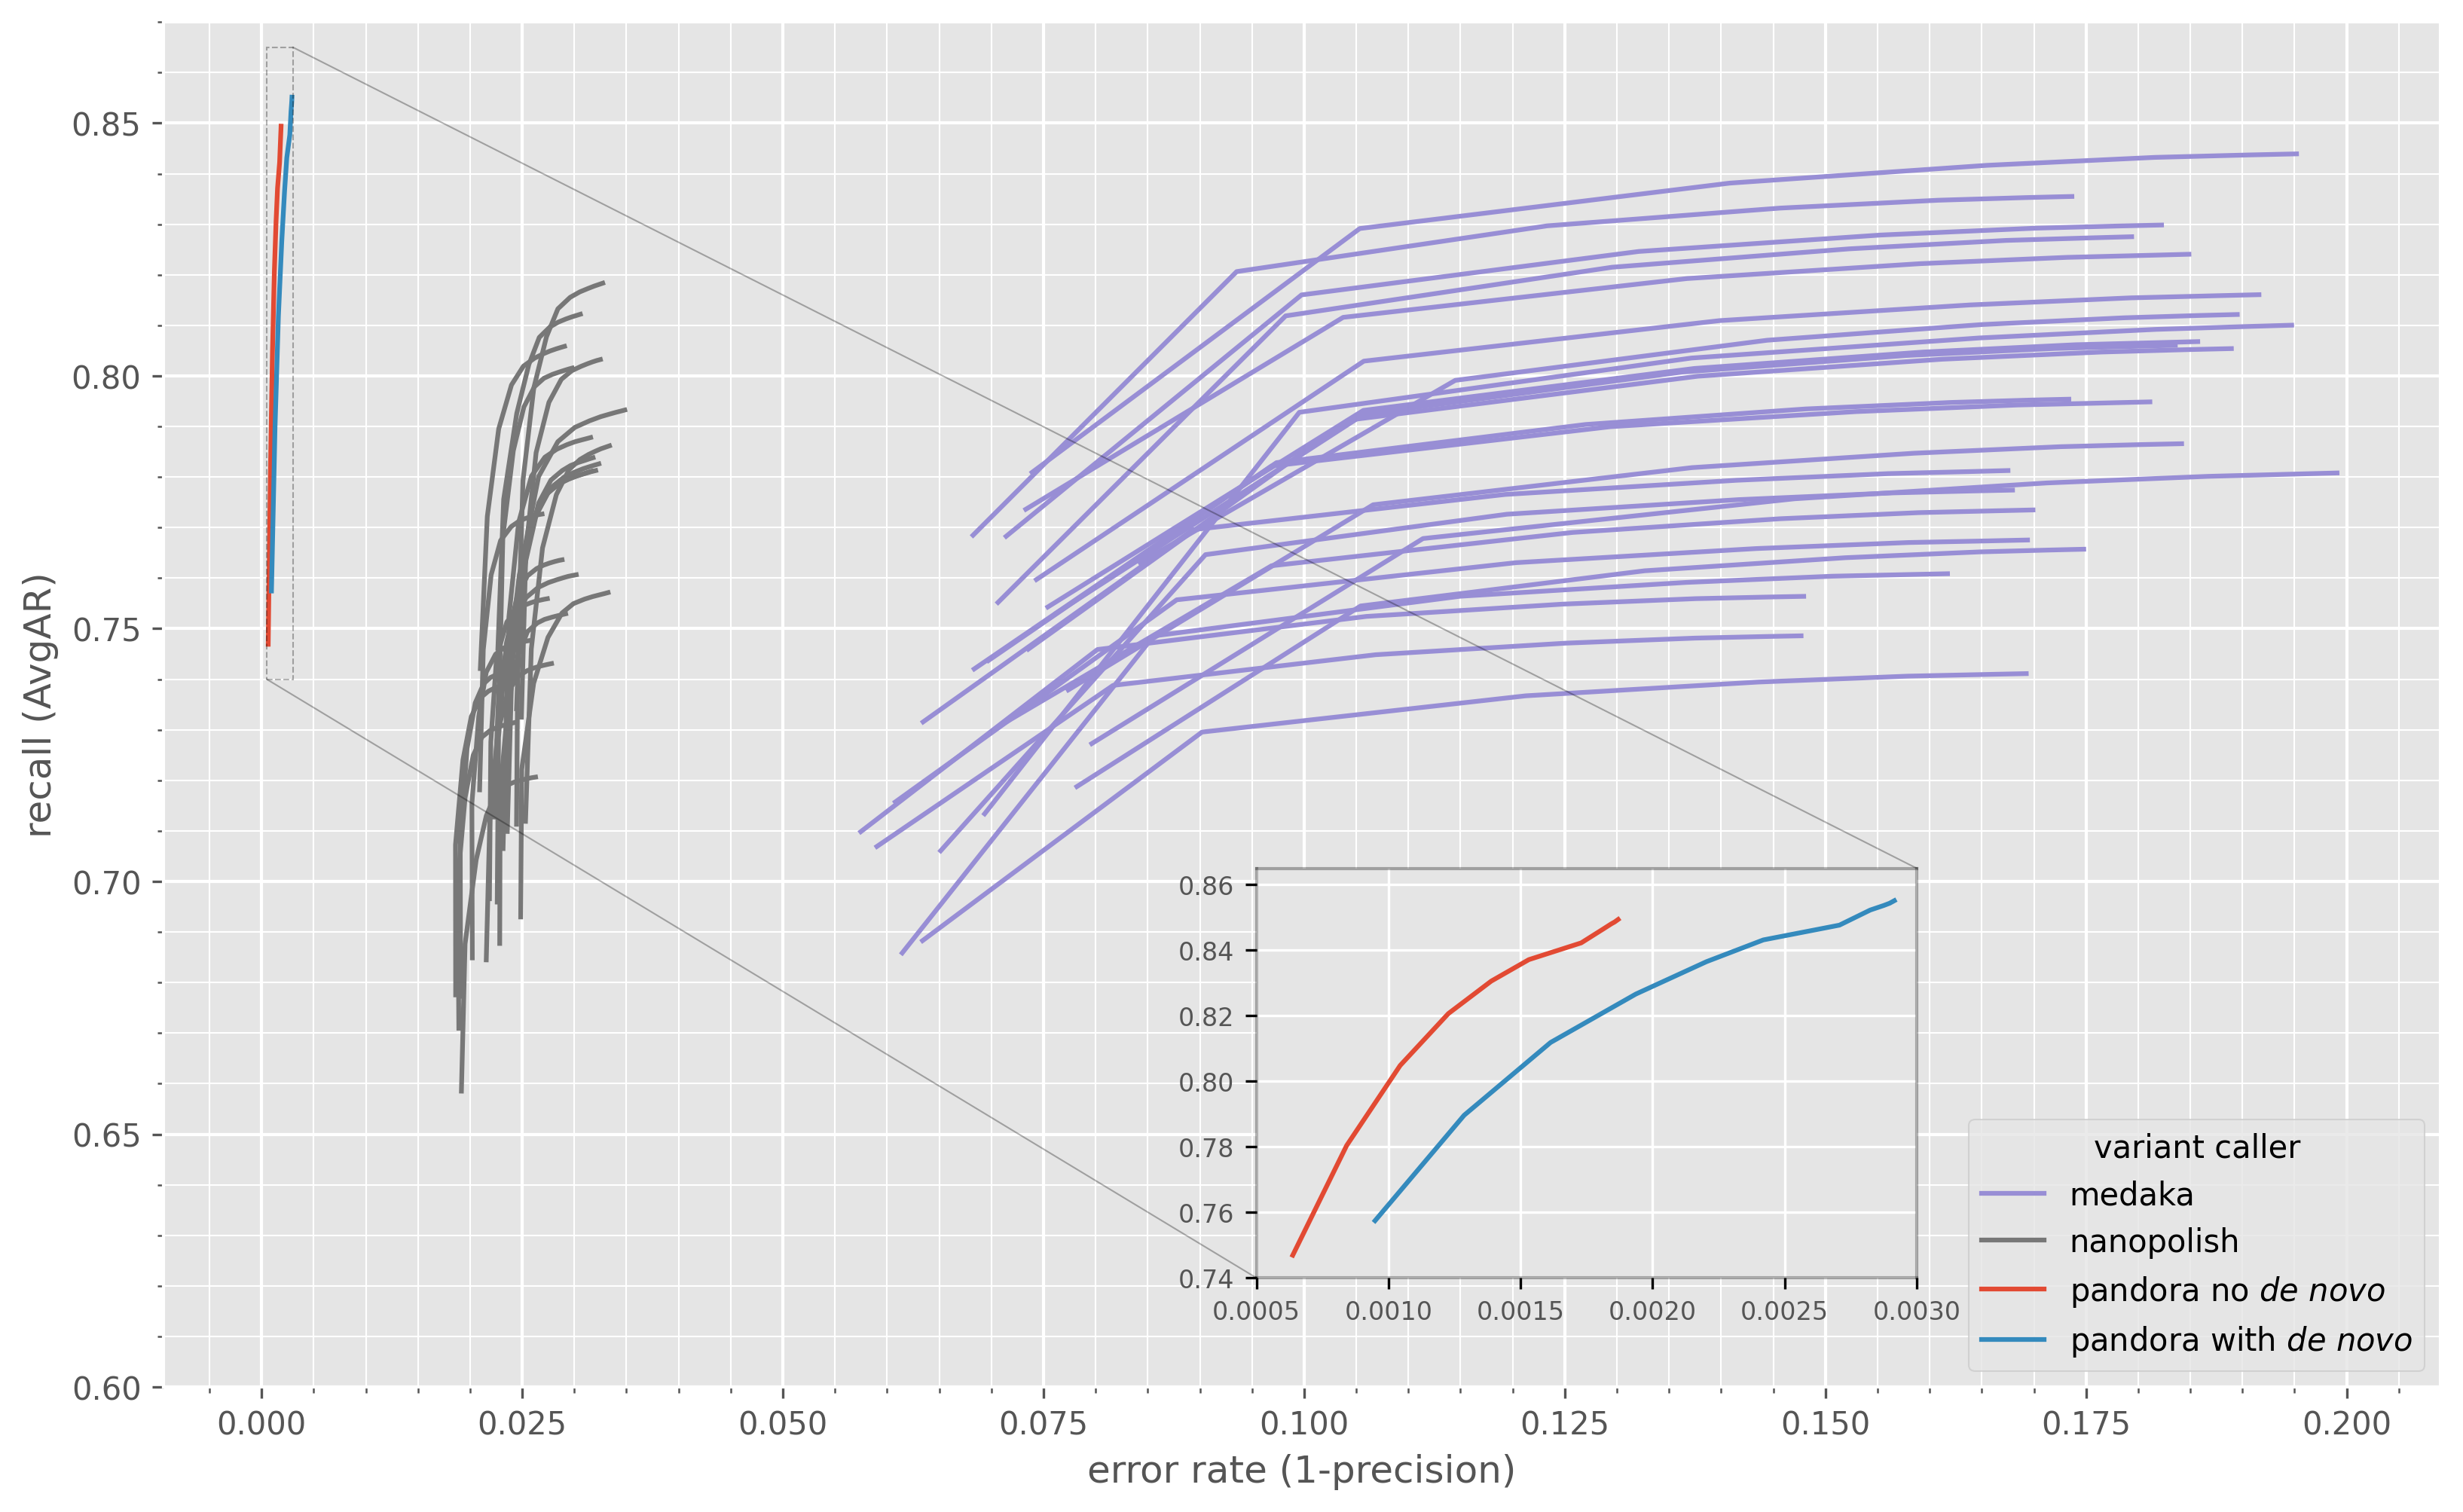
\includegraphics[width=1\linewidth]{Chapter1/Figs/nanopore_roc.png}
         \caption{\ont{}}
         \label{fig:pandora-roc-ont}
     \end{subfigure}
    \caption{Precision-recall curve for variant calls from Illumina (left; \textbf{a}) and \ont{} (right; \textbf{b}) data for different variant calling tools (colours). Each curve represents increasing genotype confidence thresholds, starting with no filtering in the top-right of each curve and increasing towards the bottom-left. \pandora{} has a single line with and without \denovo{} variant discovery, which represents the error rate and recall across all 20 samples. The other variant callers are traditional single-reference tools; therefore each line represents the use of 1/24 reference genomes from across five major \ecoli{} phylogroups. Inset windows are used to give more granularity for error rate in the best performing tools.}
        \label{fig:pandora-roc}
\end{figure}

\subsection{Summary}

In this section, using 20 diverse \ecoli{} samples we have shown that the \denovo{} variant discovery methoud outlined in \autoref{sec:denovo-method} allows \pandora{} to discover more variants (increases recall). On Illumina data it additionally improves the error rate, however on \ont{} data it appears to increase the error rate.

We also illustrated that a methylation-aware \ont{} basecalling model decreases the \pandora{} error rate - quite significantly for \denovo{} - indicating that many of the novel variants "discovered" by our method are in fact systematic technology errors.

Finally, we show that \pandora{} provides higher recall than single-reference-based variant callers for both Illumina and \ont{} data. In addition, is leads to a \ont{} error rate that is an order of magnitude lower than other tools. However, \vrb{snippy} provides lower error rates than \pandora{} on Illumina data.

% ==================================================================
\section{Discussion}
\label{sec:denovo-discussion}
%  why not just assemble best sequence in dbg?
% nearly all errors in best performing params were not within the power of de novo to discover
% a better filtering strategy than gt conf alone is needed re: sims
% ==================================================================
\section{Limitations}
\label{sec:denovo-limits}
% this is refrred to by Appendix 1 - i.e., getting stick in cycles in the dbg
% homopolymer deletions - maybe ignore them? tubby?
% variants near ends of genes
% ==================================================================
\section{Conclusion}

% ==================================================================
\section{Future Work}
\label{sec:denovo-fw}
% In future work, we plan to add indels to the simulations.
% ==================================================================
\section{Availability of data and materials}
